\chapter{\altGerEng{Implementierung}{Implementation}}


One of the primary goals of this thesis is to send text data by converting it into a visible light signal. The modulated light signal will be sent over some free distances. Then, it will be demodulated on the receiver side. The second main goal, the \ac{VLC} channel, must be designed to ensure that light can be used for \ac{EH} \cite{mahmoud2022design}.

There are multiple ways to achieve the required considerations. This thesis needs to choose paths among others to proceed. Each combination has its pros and cons. 

Principally, this thesis's implementation procedure can be divided into three parts: the theoretical approach or Methodology, component selection, and practical implementation. In this chapter, they are described. The work procedure on the Receiver side can be divided into: \ac{ID}and \ac{EH}.

\section{Methodology}
In this section of the thesis, the theoretical approach to building a prototype will be discussed.

The \ac{PS} and \ac{SS} technique will be implemented for simultaneous signal reception and \ac{EH} among many power harvesting processes. The advantage of using these splitting techniques is that they continuously harvest power from the light, even while part of the light signal is decoded in an \ac{ID} circuit. As it is constantly harvesting energy, the amount of energy stored in batteries or supercapacitors should be higher compared to the \ac{TS} Technique\cite{wang2015design}. This also means the receiver will always receive a signal at the moment it is sent and won't depend on the receiver's timing circuit. Nevertheless, the \ac{PS} technique, using the simple circuit shown in Figure \ref{fig:2.2}, is also cost-effective and less complex \cite{ma2019simultaneous}. In contrast, in the \ac{TS} complex synchronization of the time switching is necessary. For better understanding, the Theoretical Approach is subdivided into two parts: Receiver and Transmitter.

Both the transmitter and receiver will be placed in a dark, confined box that is almost free of any ambient light. This thesis's goal is to determine whether the receiver light can rely only on the light sent by the transmitter for both data communication and \ac{EH}.

\subsection{Transmitter}

Building a transmitter is the first step in creating an operational \ac{VLC} system. A computer will be used as an Information source. Through Thonny\ref{appendix:A1}, a Raspberry Pi Pico will be programmed to create a modulated Electrical signal. This electrical signal communication will follow the \ac{UART} communication method, and the modulation will be done in \ac{OOK}.

A high-power White LED will be used to transform the generated Modulated Electrical signal into the Modulated light signal \cite{7292748}. An LED driver circuit is necessary to properly run the LED, which can have high-speed switching and constant current. The Darlington pair LED circuit will be used as an LED driver, shown in Figure \ref{fig:3.2}. Since communication is done using the \ac{UART} method, the light signal will be high when no data is sent, making more light available for harvest. The Block diagram in Figure \ref{fig:4.1} shows the transmitter's working principle.

\begin{figure}
    \centering
    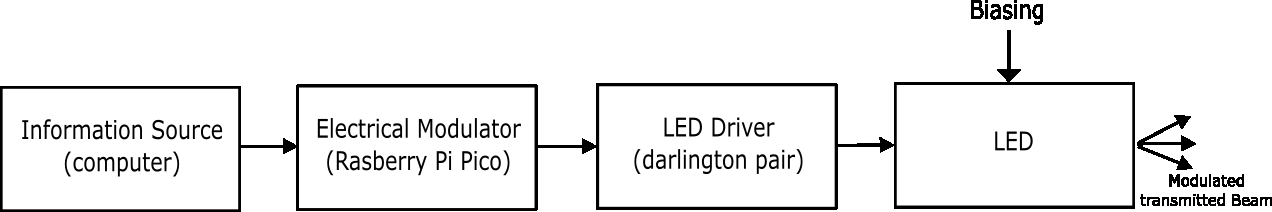
\includegraphics[width=.75\linewidth]{fig/transmitter_block.jpg}
    \caption{Block Diagram transmitter}
    \label{fig:4.1}
\end{figure}

For both power and \ac{SS}, the same transmitter configuration will be used. When multiple LED connections are necessary, the same configuration will be repeated; only LEDs will be connected in parallel. 

\subsection{Receiver}

On the receiver end, a photodetector will receive the modulated light signal sent by the transmitter. The receiver configuration will be held depending on the \ac{SLIPT} technique. 

\subsubsection{Power Splitting}

\ac{PD}s will be used as photodetectors for both \ac{EH} and data communication. Based on this thesis knowledge, since \ac{PD}s will be in \ac{PV} Mode, it will work as a small \ac{PV} cell or as a solar cell. Considering this, the thesis procedure will follow the same design procedures as the solar cell used for \ac{SLIPT}. The block diagram of the \ac{PS} Receiver configuration is shown in Figure \ref{fig:4.2} 

\begin{figure}
    \centering
    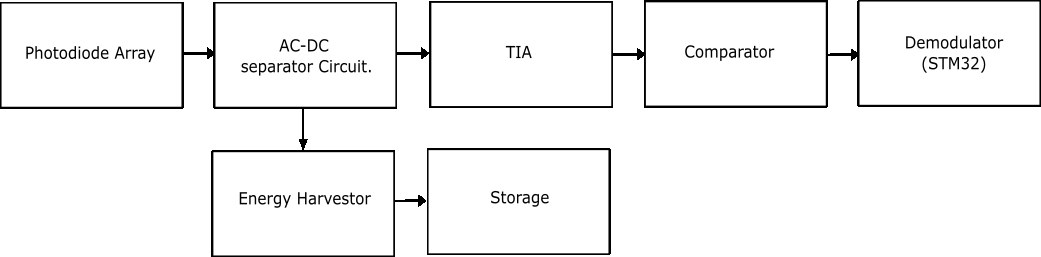
\includegraphics[width=0.75\linewidth]{fig/reciver_block_power.jpg}
    \caption{Receiver Block diagram (\ac{PS}).}
    \label{fig:4.2}
\end{figure}

The first task of designing the circuit would be to choose a suitable \ac{PD}. Since the area of the \ac{PD} is not large enough as a Solar panel, and it is not optimized to work as a Solar cell, this thesis paper proposes a novel approach of connecting multiple \ac{PD}s in series. This will add up the voltage generated while the current will remain the same \cite{gallegos2015analysis}. Based on this thesis knowledge, this method was first proposed in the paper \cite{fong2012integrated}. 

Since a \ac{PD} behaves like a solar cell in \ac{PV} mode, the equations and fundamentals should also apply to this method. The configuration of the \ac{PD} used in series is shown in Figure \ref{fig:4.3}

\begin{figure}
    \centering
    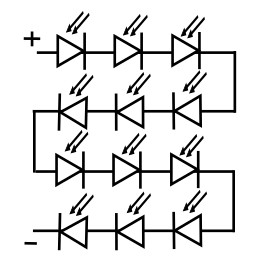
\includegraphics[width=.25\linewidth]{fig/photodiode series.jpg}
    \caption{12-\ac{PD} in series connection}
    \label{fig:4.3}
\end{figure}


There are a few benefits of having small-sized solar cells instead of larger ones. Firstly, due to a smaller area, the inherited capacitance will be small \cite{wang2015design}. Secondly, connecting cells in series will reduce the equivalent capacitance as mentioned in fundamentals. Thirdly, high \ac{SINR}s are found in large solar cells as they have a nonlinear distortion, limiting system performance. So, a bigger cell would have a terrible frequency response \cite{wang2015design}.

After choosing the \ac{PD} and its connection, work will progress to build the circuit for \ac{SLIPT}. The circuit shown in Figure \ref{fig:2.2} will be built depending on the parameters of the equivalent circuit of the series-connected \ac{PD}s. I-V characteristics of the single \ac{PD} in Photovoltaic modes need to be found first to figure out \( R_{sh} \), and \( R_{s} \) \cite{wang2015design}. An I-V curve can be plotted by measuring Voltage and Current for each operating point. Two starting points can already be considered:  Short Circuit Current and Open Circuit Voltage \cite{gallegos2015analysis}. So, varying load, I-V combinations can be found \cite{fong2012integrated} and plotted. However, it needs to be kept in mind that, since LED is used, the light intensity values will also be lower.

Putting \( I_{D} \) from equation \ref{eq:3.2} into equation \ref{eq:3.1} , the current becomes:

\begin{equation}
\ I = I_{ph}-I_{0}exp\left[ \frac{(V + IR_{s})}{n_{s}V_{T}}-1\right]-\frac{(V + IR_{s})}{R_{sh}} \
\label{eq:4.1}
\end{equation}

\( R_{sh} \) and \( R_{s} \) can be found from the slope of the I-V curve \cite{badi2021accurate}. The current derivative defines the slope with respect to voltage, which is applicable under any operating conditions. So, the equation \ref{eq:4.1} is derived with respect to voltage to find out \( R_{sh} \)  and \( n_{s} \) \cite{gallegos2015analysis}:

\begin{equation}
\ \frac{dI}{dV} = -\frac{I_{0}}{V_{T}}exp\left[ \frac{(V + IR_{s})}{V_{T}}\right](1+R_{s}\frac{dI}{dV})-\frac{1}{R_{sh}}-\frac{ R_{s}}{R_{sh}}\frac{dI}{dV} \
\label{eq:4.2}
\end{equation}

Rearranging, 

\begin{equation}
\ \frac{dI}{dV}(1 +\frac{R_{s}}{R_{sh}} + \frac{I_{0}R_{s}}{V_{T}}exp\left[ \frac{(V + IR_{s})}{V_{T}}\right])   = -\frac{I_{0}}{V_{T}}exp\left[ \frac{(V + IR_{s})}{V_{T}}\right]-\frac{1}{R_{sh}} \
\label{eq:4.3}
\end{equation}

Then, considering the short circuit condition \(V = 0\) and  \(I = I_{sc} \),

\begin{equation}
\ I_{0}exp\left[ \frac{(V + IR_{s})}{V_{T}}\right]= I_{0} exp\left[ \frac{I_{sc}R_{s}}{V_{T}}\right] \approx 0  \
\label{eq:4.4}
\end{equation}
 
assuming \( R_{s} \) is minimum comparing to \( R_{sh}\) and \( I_{0} \) is in nano Ampere range \cite{badi2021accurate}, 

\begin{equation}
\ \frac{dI}{dV} = -\frac{1}{R_{sh}} \
\label{eq:4.5}
\end{equation}

Similarly, \( R_{s} \) can be found from equation \ref{eq:4.3} when the Open circuit condition is regarded, \(I = 0\) and \(V = V_{oc}\), 

\begin{equation}
\ I_{0}exp\left[ \frac{(V + IR_{s})}{V_{T}}\right]= I_{0} exp\left[ \frac{V_{oc}}{V_{T}}\right] = I_{sc}  \
\label{eq:4.6}
\end{equation}

Then equation \ref{eq:4.3} becomes,

\begin{equation}
\ \frac{dI}{dV}(1 +\frac{R_{s}}{R_{sh}} + \frac{I_{sc}R_{s}}{V_{T}})   = -\frac{I_{sc}}{V_{T}}-\frac{1}{R_{sh}} \
\label{eq:4.7}
\end{equation}

As \( R_{sh}\) is large, it can be assumed that \( 1/R_{sh}\) and \( R_{s}/{R_{sh}}\) are negligible, then the equation can be represented as \cite{badi2021accurate},

\begin{equation}
\ R_{s} = - \frac{dV}{dI} - \frac{V_{T}}{I_{sc}} \
\label{eq:4.8}
\end{equation}

The slope (\( dI/dV\)) of the I-V curve can be found both in short and open circuit conditions, and putting them in this equation \( R_{s} \) and  \( R_{sh}\) can be finally found.

Capacitance C can be found from the datasheet of the \ac{PD}. The value of the wiring and connection induction is estimated at 120nH in the paper \cite{wang2015design}. This thesis will do the same.

To find out the small signal resistance, the equation below can be used \cite{sze2021physics}:

\begin{equation}
\ r = \frac{V_{T}}{I_{0}} \ = \frac{nKT}{qI_{0}} \
\label{eq:4.9}
\end{equation}

\( I_{0} \)  is the reverse current of the diode, also called the dark saturation current, which can be found from the data sheet of the \ac{PD}. 

Equation for equivalent C, \( R_{sh} \), and \( R_{s} \) are already shown.  Since it is also a parallel resistance, the equivalent resistance equation of small signal resistance should be: 

\begin{equation}
\ r_{eq} =\frac{Ns}{Np}r \
\label{eq:4.10}
\end{equation}

With the equivalent circuit parameters, synchronous \ac{EH} and data communication circuit becomes like the Figure \ref{fig:4.4}.

\begin{figure}
    \centering
    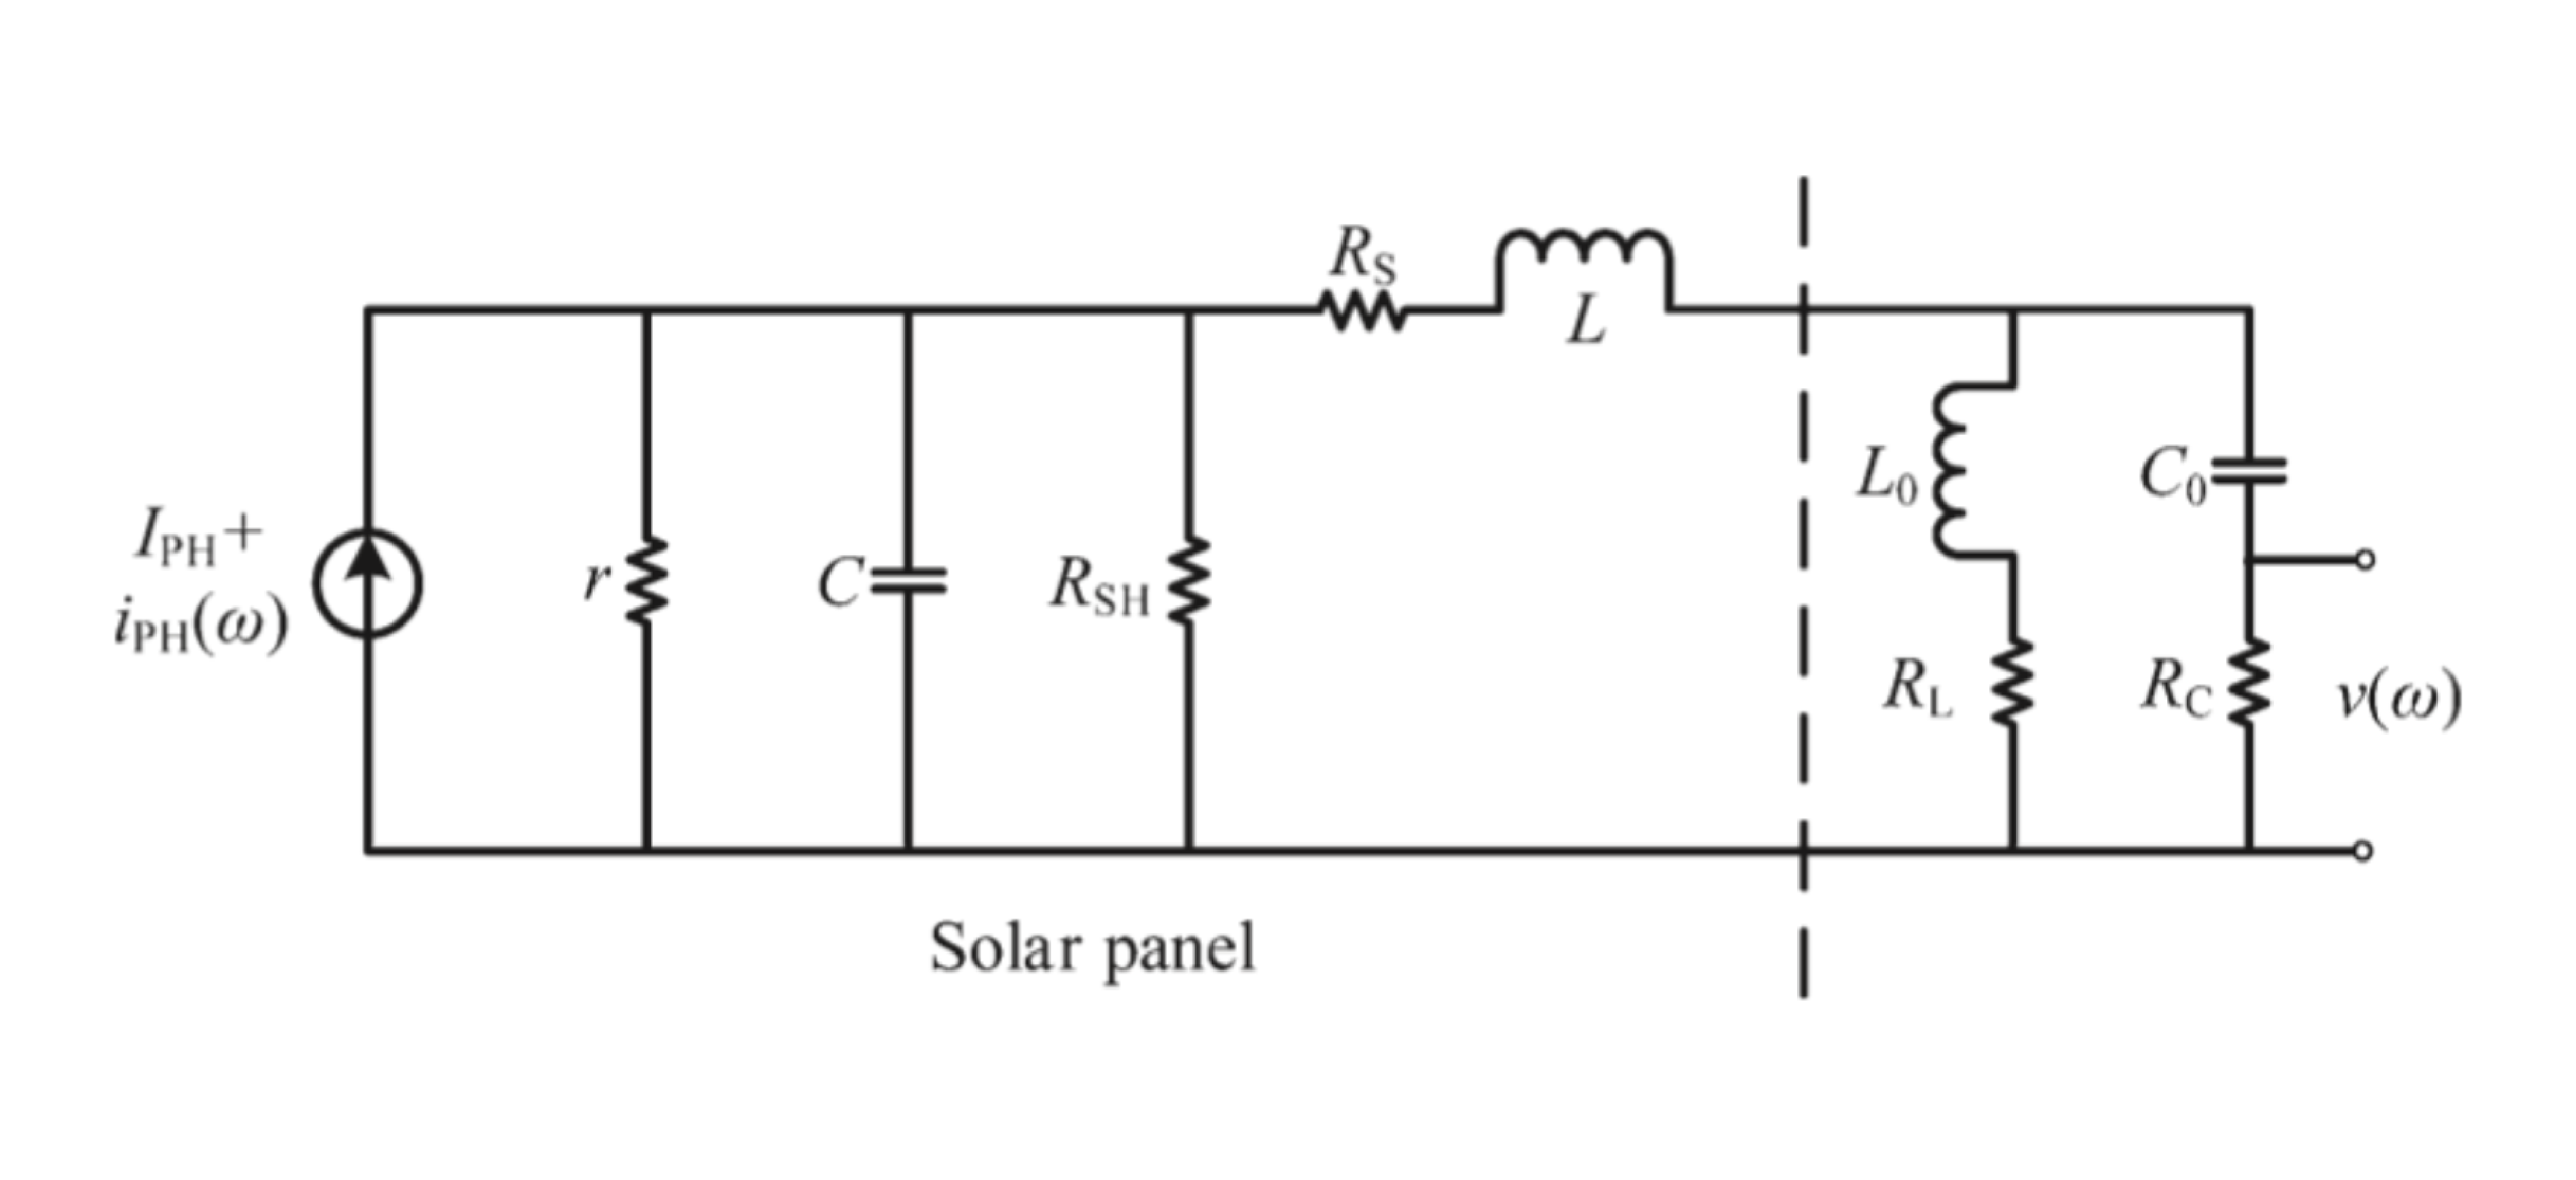
\includegraphics[width=0.75\linewidth]{fig/equivalentcircuit.pdf}
    \caption{Series connected \ac{PD} equivalent circuit for SPLIT}
    \label{fig:4.4}
\end{figure}

As five unknown parameters of the circuit: C, \( R_{sh} \), \( R_{s} \), r, and L are found out. The next step would be determining the parameters of the \ac{EH} and Communication branches. For \ac{EH}, the optimal load for a particular irradiance must be found. When light irradiance increases, the load for \ac{EH} decreases. Optimum load \( R_{L} \) can be determined using the p-v curve, taking into account the specific light irradiance and the DC component of the optical information signal \cite{wang2015design}. \( R_{L} \) and  \( L_{0} \) together build a low-pass filter and will allow only the DC part of the received signal. But a larger inductor value can better block the AC signal \cite{wang2015design}. The value of \( L_{0} \) and other circuit parameters will also depend on light irradiance. Although the value of \( L_{0} \) doesn't have an effect on high frequency for the channel response of the communication branch\cite{wang2015design}.

This thesis proposes to use LTSpice to find the optimum value of the  \( R_{L} \) and \( L_{0} \). A parameter sweep of the \( R_{L} \) for multiple \( L_{0} \) to find out a better frequency response at low frequency can be used. Another approach would be a DC parameter sweep of the \( R_{L} \) for multiple \(L_0 \) to find out the P-V curve and use the \ac{MPPT} point for optimum values.

In the Communication branch \( R_{c} \) and \( C_{0} \), they together build a high-pass filter and will allow only the AC part to pass through it, which will be used for Data communication later. The paper \cite{wang2015design} showed how \( R_{c} \) and \( C_{0} \) are found using frequency response curve. The author concluded that the frequency response increases, although the -3 dB bandwidth decreases with the increase of the resistor \( R_{c} \). It was found that higher \( C_{0} \) will reduce DC ripples in low frequencies, improving channel response. However, it will also reduce gain, which is unwanted in the frequency response. Hence, an optimum value that balances both \cite{wang2015design} needed to be found.  

This thesis proposes to use LTSpice to find the optimum value of the  \( R_{c} \) and \( C_{0} \). A parameter sweep of the \( R_{c} \) for multiple \( C_{0} \) to find out the better frequency response at high frequency can be used. 

After finding these circuit parameters, an \ac{ID} circuit would be added across the \( R_{c} \). This \ac{ID} circuit would also contain a voltage amplifier, a comparator, and a demodulator. The voltage amplifier will amplify the voltage signal. The comparator circuit will convert the signal into a near-digitized signal. The design of the comparator is similar to the amplifier's design with a Bias network, but it will not have a feedback resistor. At last, this signal will be fed into a demodulator microcontroller like STM32. At first, this circuit will run on the power supply from outside, which means a bias voltage will be provided, to see if this \ac{ID} circuit can decode the signal sent by the transmitter. 

When the signal sent by the transmitter is detected without any concern, the procedure will move to build the \ac{EH}. Power Management is necessary \cite{fong2012integrated}, which will take the place of \( R_{L} \) as a load. This Power management will consist of a boost circuit. Boosted power will be stored in a supercapacitor. A supercapacitor is chosen because of its fast charging and discharging ability. Power management will also ensure the supercapacitor is charged up in a controlled way with constant voltage. The power management will also contain a buck converter to maintain the output feed to the \ac{ID} circuit. This buck converter will always ensure a constant Bias voltage is provided to the voltage amplifier and the comparator, as well as supply power to run the STM32 module.

\subsubsection{Space Splitting}

\ac{PD}s will also be used for the \ac{SS} \ac{SLIPT} technique. However, with \ac{PS}, the fundamental difference is that here, a \ac{PD} can be either photoconductive or photovoltaic mode, which will be used for the communication branch. However, since power will be supplied from harvested energy, building reverse bias voltages is complicated and power-consuming. So, this thesis work chooses the photovoltaic mode. However, it will make the receiver slower. Nevertheless, other \ac{PD}s must be used in photovoltaic mode, since they will be used for \ac{EH}. Most research on \ac{SS} techniques \cite{ma2019simultaneous} has utilized solar panels for \ac{EH} and \ac{PD}s for communication. This thesis aims to explore the potential of using \ac{PD}s as an \ac{EH} tool, similar to the approach taken in \cite{de2024reconfigurable} in its Single \ac{PD} mode. This thesis also aims to compare and try to differentiate the main differences between solar panels and \ac{PD}s as \ac{EH} sources. The block diagram of the \ac{SS} receiver configuration is shown in Figure \ref{fig:4.5}.

\begin{figure}
    \centering
    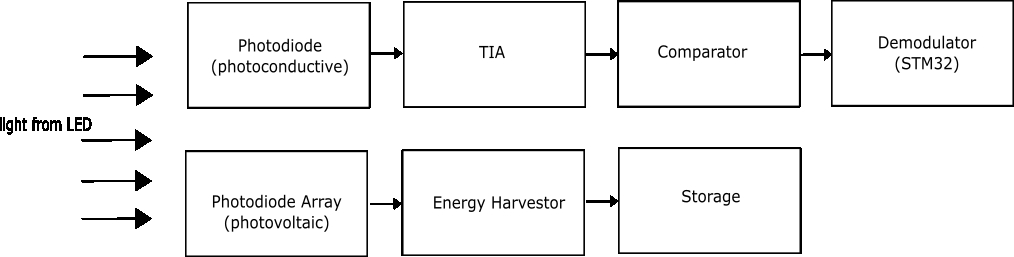
\includegraphics[width=0.75\linewidth]{fig/reciver_block_space.jpg}
    \caption{Receiver Block Diagram (\ac{SS}).}
    \label{fig:4.5}
\end{figure}

The \ac{ID} circuit will consist of a \ac{TIA}, a comparator, and a demodulator. The voltage amplifier will amplify the voltage signal, and the design consideration shown in Figure \ref{fig:3.10} is taken for designing the circuit.

A rail overshoot protection can be added to the \ac{TIA}'s feedback loop. It will protect the \ac{TIA} circuit if a massive amount of light falls on the \ac{PD}, generating a current signal impulse. Three JFETs connected as diodes can be used for overshoot protection.

Then the ambient filter connected to the output of the \ac{TIA} will reduce the effect of the outside light and other noises. The comparator circuit will convert the analog signal from the amplifier into a near-digitized signal. The design of the comparator is similar to the design of the \ac{TIA} with a Bias network, but without a feedback resistor. At last, this signal will be fed into a demodulator microcontroller like STM32. 

At the beginning, this circuit will run on the power supply from outside, which means a bias voltage will be provided, to see if this \ac{ID} circuit can decode the signal sent by the transmitter. When the signal sent by the transmitter is detected without any concern, this thesis work will move to build the \ac{EH}.

In the paper \cite{de2024reconfigurable}, the \ac{PD}s used for the energy harvest are all connected in series, but they used a LASER for data communication and a 60W incandescent lamp energy projection. Since the intensity of LASER light is much higher, its voltage, current, and power will also be higher \cite{de2024reconfigurable}.

More current can be generated by connecting them in parallel or by increasing the light intensity, and this can also be done using more LEDs or a laser instead \cite{de2024reconfigurable}. A novel configuration of \ac{PD}s is suggested by this thesis and shown in Figure \ref{fig:4.16}. This thesis will also compare the solar cell as a harvesting unit. When using Solar, it will be directly connected to the power management unit.

\begin{figure}
    \centering
    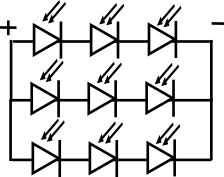
\includegraphics[width=0.25\linewidth]{fig/photodiode_connection.png}
    \caption{New Photodiode Connection}
    \label{fig:4.16}
\end{figure}

Similar to the \ac{PS}, this Power management will consist of a boost circuit and a buck converter. Power will be stored in a supercapacitor. Power management will also ensure the supercapacitor is charged up in a controlled way to ensure it will not over-charge or under-charge. The buck converter will ensure a constant Bias voltage is always provided to the \ac{TIA}, comparator, and supply power to run the STM32 module. 

\section{Component Selection}

\subsection{Electrical Modulator}

Arduino UNO could be used as an Electrical modulator, as it is used in paper \cite{mahmoud2022design}. An STM32 board could also be used as a building material for the transmitter. For example, STM32F4discovery is used in \cite{7420990} as an ADC converter to send a 3.3V \ac{USART} signal to the LED driver circuit.

A Raspberry Pi board can also be used as an Electrical Modulator. Raspberry Pi Pico WH is a low-cost but flexible RP2040 development platform. It has all the features of Pico plus a 2.4GHz wireless interface. Raspberry Pi Pico WH generates a modulated pulse signal command to an LED to produce the required frequency signal. Pi Pico WH has a built-in hardware \ac{UART} pin (UARTO TX) at pin 0, which this thesis aims to use for \ac{UART} data communication. This signal will then be imposed upon the \ac{PD}. The general voltage level of the pins of the pico board is 3.3V. It was chosen for this thesis work because of its flexibility. It can be programmed by Thonny\ref{appendix:A1} to produce \ac{UART} signal of different baud rates. 


\subsection{LED}

A 60-W incandescent lamp (Reflector R80) was used to evaluate the \ac{EH} capability using an artificial light source and three different color LASERs for data communication in paper \cite{de2024reconfigurable}.

Since \ac{EH} is one of the primary goals, and harvested power depends on the intensity of the light, which in turn depends on the power of the LED, it is better to choose an LED with more power. For this thesis, the main requirements of an LED of the transmitter are built based on the paper \cite{mahmoud2022design}, and are shown in Table \ref{tab:4.1}.

In search of the powerful LED with this characteristic, the thesis work came across the XLamp® XB-D LEDs used in paper \cite{7292748}. The manufacturing company is Cree LED. They are new high-performance LEDs with a small footprint design (2.45 mm x 2.45 mm x 1.84 mm). They are available in many color combinations and low cost \cite{productfamily} with a viewing angle of 115 degrees. 
An XB-D Neutral White LED with 4750 K 75-CRI has been chosen for the thesis work since it follows the requirement shown in Table \ref{tab:4.1}. It has an electrically neutral thermal path and is Reflow solderable.

The main characteristics of this LED are shown side by side with the required characteristics in Table \ref{tab:4.1}.

\begin{table}
    \centering
    \caption{Parameters comparison of the LED}
    \begin{tabular}{|c|c|c|c|c|}
         \hline
         \textbf{Parameters} &\textbf{Requirement}  &
         XB-D Neutral White LED\\
         \hline
         Color temperature  &3000-3200K(Warm White) &4750 K\\
         \hline
         Forward current  &700mA  &1A(max)\\
         \hline
         Luminous flux  &180-200LM &114 lm \\
         \hline
         Forward voltage &3.3 - 3.6V  &2.9 - 3.3 \\
         \hline
         Reverse voltage  &5V   &5V\\
         \hline
         Power &3W   &3W\\
         \hline

    \end{tabular}
    \label{tab:4.1}
\end{table}


\subsection{LED Driver}
Paper \cite{thongsa2018design} uses an LED driver circuit (ULN2560N) for building the transmitter. An LED driver, TLC5916, was used in paper \cite{6757172} for driving the LED array. Paper \cite{7420990} used a combination of TLP250 photo-coupler driver and IRF740 N-MOSFET for fast switching and high response time. A Darlington pair consisting of two transistors(BC547), shown in Figure \ref{fig:3.2}, will be used in this thesis for fast switching.


\subsection{Photodiode}
In paper \cite{de2024reconfigurable}, nine red-enhanced high-performance silicon (Luna Optoelectronics sd445-14-21-305) PDs were arranged in a 3 × 3 matrix with minimal spacing between the packages. Their active area was 1 \(cm^{2}\). It has 100\(mm^{2}\) large active area, which makes it great for \ac{EH}, but it also makes it slower. 45 ns with reverse bias or 190ns (without bias)  \cite{passion}. Important parameters are shown in Table \ref{tab:4.2}.

BPW34, a silicon PIN \ac{PD}, has been chosen for the thesis as a \ac{PD} and energy harvester because it has High Photosensitivity with a 7.5 \(mm^{2}\) miniature compact design. It has a clear epoxy package and light can quickly enter the capture zone. It can capture both Visible and near-infrared radiation. The range of its spectral bandwidth is 430nm to 1100nm \cite{intertechnology2011bpw34}.

BPW34 has a speedy response time. Other key specifications include a reverse voltage of 60V, low dark current, small junction capacitance, and peak sensitivity at 900 nm, making it ideal for high-speed photodetectors and optical sensing applications \cite{intertechnology2011bpw34} \cite{7420990}.

BPW34 can be used for \ac{EH}. Its Open circuit voltage (\(V_{oc}\)) is 350 mV, and it is small, making it convenient to use in series. Six of the BPW34 will generate about 2V, and ten will produce 3.5V, but the current will remain the same, as a single \ac{PD}. The amount of illumination will determine this. According to the datasheet, reverse light current has a proportional relationship with illumination and irradiance. It remains comparatively constant with temperature changes. Another important parameter is short circuit current (\(I_{sc}\)). \cite{intertechnology2011bpw34}

The key features are shown in the table \ref{tab:4.2}for a comparison with sd445-14-21-305. 

\begin{table}
    \centering
    \caption{Parameters of the Photodiode}
    \begin{tabular}{|c|c|c|c|c|}
         \hline
         \textbf{Parameters} &\textbf{BPW34} &\textbf{sd445-14-21-305}  \\
         \hline
         Reverse dark current  &2 nA &6 nA \\
         \hline
         Diode capacitance  &70 pF  &500 pF\\
         \hline
         Open circuit voltage  &350mV &\\
         \hline
         Detector area of PD &7.5\(mm^2\) &100\(mm^2\) \\
         \hline
         Reverse light current  &50\(\mu A\)  & \\
         \hline
         Angle of half sensitivity \(\phi\)  & \(\pm\)60 &\\
         \hline
         Range of spectral bandwidth   &430 to 1100nm &max 900nm \\
         \hline
         Response Time &20ns 100ns rise/fall &45ns\\
         \hline
         Breakdown voltage  &60V  &50V\\
         \hline
         Short Circuit current  &47\(\mu A\)   &\\
         \hline
    \end{tabular}
    \label{tab:4.2}
\end{table}

\subsection{Solar Panel}
Paper \cite{fan2017circuit} used a solar cell named KXOB22-12X1L as a Photovoltaic cell for \ac{PS}. For a similar goal, paper \cite{wang2022high} used SC-9728 with an open voltage of 6V and a short circuit current of 15 mA.

To check the \ac{EH} capability, a small solar panel (SKU 313070004) made of single-crystal material has been chosen because of its higher conversion efficiency of 17\%. Detailed 
features are shown in the table \ref{tab:4.3}.

\begin{table}
    \centering
    \caption{Parameters of the Solar Panel}
    \begin{tabular}{|c|c|c|c|c|}
         \hline
         \textbf{Parameters} &\textbf{SKU 313070004}  \\
         \hline
         Power Rating  &0.5W   \\
         \hline
         Dimensions  &70x55x3(±0.2) mm  \\
         \hline
         Typical voltage  &5.5V  \\
         \hline
         Open circuit voltage  &8.2 V \\
         \hline
         Maximum load voltage &6.4 V  \\
         \hline
    \end{tabular}
    \label{tab:4.3}
\end{table}


\subsection{Amplifier}

In paper \cite{7420990}, the LM353 IC is used as a non-inverting amplifier. But this would not be suitable for an energy-efficient \ac{Li-Fi} receiver, because it requires a higher dual supply voltage (±15 V) and high input bias current of 50pA. Moreover, it has only 4 MHz Gain Bandwidth Product and a slew rate of 13V/\(\mu\)S \cite{LM353}.


Opa355 was considered as a \ac{TIA}for the thesis. Since the planned output of the Power Management would be around 3 to 3.5, it is better to use an \ac{OPAmp} for \ac{TIA}, whose operation is in this range. The \ac{OPAmp}'s operation range is 2.5 to 5.5V \cite{sbos195}. In addition, it has a low input bias current, 3pA, and provides rail-to-rail output, which will help maximize signal swing in low-voltage systems. Opa355 has a high bandwidth of 200MHz, which is excellent for a high-speed \ac{VLC} system. The common-mode input range for OPA355 extends 100 mV below ground and goes up to 1.5 V from V+. The output swing is within 100 mV of the rails, allowing for a wide dynamic range \cite{sbos195}.

OPA380 is another great candidate, having 90MHz Gain Bandwidth and was also used in paper \cite{de2024reconfigurable}. The supply range for this \ac{OPAmp} is 2.7 to 5.5V. OPA380 is designed to be robust with high precision and low noise. Due to this, the measurement of signal currents on the order of 1nA and up to 100 \(\mu\)A in a single I/V conversion stage is possible \cite{monitoring_2003}. It is suited for fast control loops and wideband \ac{PD} transimpedance amplifiers. The electrical Characteristics of these \ac{TIA} are compared in the table \ref{tab:4.4}

\begin{table}
    \centering
    \caption{Parameters of OpAmps}
    \begin{tabular}{|c|c|c|c|c|}
         \hline
         \textbf{Parameters} &\textbf{OPA355 } &\textbf{OPA380}
         \\
         \hline
         Supply Voltage Range  &2.5 V – 5.5 V  &2.7 V – 5.5 V\\
         \hline
         Gain Bandwidth Product (GBW)  &200 MHz  &90 MHz\\
         \hline
         Slew Rate  &360 V/\(\mu\)s &80 V/\(\mu\)s  \\
         \hline
         Input Bias Current &~3 pA  &3–50 pA \\
         \hline
         Input Offset Voltage  &±2 mV   &25 \(\mu\)V max\\
         \hline
         Common-Mode Voltage Range &(V-)-.1V  \(<V_{CM} <\) (V+) - 1.8V&(V-)\(<V_{CM} <\)(V+) - 1.8V\\
         \hline
         Input Voltage Noise Density  &5.8 \(nV/\sqrt{Hz}\)  &5.8 \(nV/\sqrt{Hz}\)\\
         \hline
         Output Voltage Swing (3.3V Vcc)  &~0.1 V to 3.2 V   &~0.1 V to ~3.0 V\\
         \hline
    \end{tabular}
    \label{tab:4.4}
\end{table}


\subsection{Comparator}


Paper \cite{6757172} used TLV2782 as a comparator while paper \cite{7420990} considered LM393 to compare the signal after amplification to eliminate signals below 1V. However, LM393 has a lower response time and is not suitable for high-speed digital signals. 

A comparator in the supply range of 2.7V to 5.5V is needed to transform the \ac{TIA}'s output into the digital domain. The supply range of Omamp-based TLV3201 is 2.5 V – 5.5 V, which perfectly aligns with the requirement. It has 1.2 mV of internal hysteresis for improved noise performance, with an input common-mode range that extends 200 mV. The main factor behind choosing TLV3201 is that it has low power consumption (40 \( \mu \)) and a quick response time (40ns). Nevertheless, it has a small package in SOT-23(5) with features such as rail-to-rail inputs, low offset voltage (1 mV), and large output drive current \cite{sbos561}. Detailed 
features are shown in the table \ref{tab:4.5}

\begin{table}
    \centering
    \caption{Parameters of the Solar Panel}
    \begin{tabular}{|c|c|c|c|c|}
         \hline
         \textbf{Parameters} &\textbf{TLV3201}  \\
         \hline
         Supply Voltage Range  &2.5 V – 5.5 V  \\
         \hline
         Response time  &40ns  \\
         \hline
         Power consumption  &40 \( \mu \)  \\
         \hline
         Common-mode voltage &+200 mV to -200 mV \\
         \hline
         Input Bias Current &~1 pA  \\
         \hline
    \end{tabular}
    \label{tab:4.5}
\end{table}



\subsection{Power Management}

In the paper \cite{de2024reconfigurable}, an ultra-low-power boost converter with a battery management system (Texas Instruments BQ25504 EVM) controls the \ac{EH} process. The BQ25504 is specifically made to efficiently collect and maintain the power generated from various DC sources, and it has an integrated dynamic maximum power point tracking for optimal energy extraction.

For this thesis work, BQ25570 is selected as it has both a nano power boost charger and a buck converter for energy harvester-powered applications. 

The BQ25570 is an integrated \ac{EH} Nano-Power management solution that is well suited for meeting the special needs of ultra-low power applications. The product is specifically designed to efficiently acquire and manage the microwatts (\textmu W) to milliwatts (mW) of power generated from DC sources like photovoltaic (solar) or thermal electric generators\cite{slusbh2}, which is vital for our thesis. BQ25570 has a cold start circuit built in, a hysteretic boost converter with lower efficiency than the main boost charger. Its functionality is to boost the main booster charger above 1.8V to run in normal operation mode \cite{slusbh2}.

To evaluate the thesis design and build the first proof prototype, this thesis will use an \ac{EVM} named Solar Energy Click(MIKROE-2814). This \ac{EVM} board uses BQ25570 and follows the design considerations provided in the BQ25570 datasheet.

The \ac{EVM} can recharge a Lithium-Ion battery or other storage system (ex: supercapacitor) through its Battery Output points or hold a charge in its built-in 220mF supercapacitor. Moreover, it provides continuous power to devices using stored energy through its Output pin. So, the connected load can be powered by the connected storage or a supercapacitor soldered on the board. This \ac{EVM} is a perfect fit for use as a power management system for wireless sensor networks and, hence, for \ac{VLC} systems \cite{solar}.

It has undervoltage and overvoltage protection for the storage/Battery. When the storage voltage drops under 2.85V, the load is disconnected from the storage. Again, the storage will not be overcharged above 4.06V as it will disconnect the voltage input from the Battery. Moreover, the nano-power management system provides proper charging conditions for the storage by maintaining a constant voltage of 3.25V\cite{solar}. It will stop powering the load when the voltage drops below 1.95V. This prevents damage by completely draining out of the connected storage element, by turning off the buck converter \cite{solar}\cite{slusbh2}. Another critical factor is the \ac{EH} input terminal power rating, which must be a minimum of .005mW and a Maximum of 510mW\cite{solar}. The table \ref{tab:4.6} shows the most critical parameters of the \ac{EVM}.

\begin{table}
    \centering
    \caption{Parameters of the EVM}
    \begin{tabular}{|c|c|c|c|c|}
         \hline
         \textbf{Parameters} &\textbf{Solar Click (EVM)}  \\
         \hline
         Input Voltage Rating  &0.1V(min) to 5.1V(max)  \\
         \hline
         Input Terminal Power  &.005mW(min) to 510mW(max)  \\
         \hline
         Output Voltage  &2.6V \\
         \hline
         Output Current &100mA  \\
         \hline
         Built-in supercapacitor  &200 mF  \\
         \hline
         Undervoltage protection  & 1.95v \\
         \hline
         Overvoltage protection  & 4.06v \\
         \hline
    \end{tabular}
    \label{tab:4.6}
\end{table}
 

\subsection{Super Capacitor}

In paper \cite{de2024reconfigurable}, a 5V 0.1-F supercapacitor(EATON PB B3-129) was used as an energy storage device. A 100F super/ultracapacitor from MAXWELL Powercache is used for storing energy in \cite{simjee2006everlast}.

The KEMET 5.5V .1F supercapacitor can be used as a secondary battery as a power backup in a DC circuit where low-voltage applications are required. For this thesis, it is chosen because it can charge up within a few seconds and can be charged/discharged for a lifetime \cite{supercap}. This FT series supercapacitor (FYD0H104ZF), also known as electric Double-Layer Capacitors (EDLCs), uses an electrolyte in a sealed container. The table \ref{tab:4.7} shows the most critical parameters of the supercapacitor.

\begin{table}
    \centering
    \caption{Parameters of the supercapacitor}
    \begin{tabular}{|c|c|c|c|c|}
         \hline
         \textbf{Parameters} &\textbf{supercapacitor (FYD0H104ZF)}  \\
         \hline
         Temperature Range  &-25°C to +70°C  \\
         \hline
         Maximum Operating Voltage  &5.5 VDC  \\
         \hline
         Capacitance  &0.10F(Charge) 0.10F(Discharge) \\
         \hline
         Equivalent Series Resistance (ESR) &100\(\Omega\)  \\
         \hline
         Current (30 minutes after charging)  &0.15 mA   \\
         \hline
         Voltage Holding Characteristic Minimum  & 4.2v \\
         \hline
    \end{tabular}
    \label{tab:4.7}
\end{table}


\subsection{Demodulator}

In paper \cite{de2024reconfigurable}, the firmware of the main \ac{MCU}, STM32L4R9, ultra-low-power, was done in C++, using STMCube Integrated Design Environment (IDE)\ref{appendix:A2} for the STM32. Paper \cite{7420990} used the STM32F4 Discovery board for signal processing, especially its DAC feature. 

In this work, an STM32-Nucleo Board will be used as a demodulator. The particular model name is STM32-Nucleo L011k4. It has 16 KB of Flash memory. It can work in Power saving mode, and it's an affordable way to build the prototype required for this thesis work. This STM32 Board can be powered in four ways, but this thesis wishes to use +3V3 power supply pins on CN4.

STM32-Nucleo L011k4 has a \ac{USART} virtual COM port,  available on PA2 (TX) and PA15 (RX). They can be connected with the ST-LINK/V2-1 by SB2 and SB3. Except for this, only one \ac{USART} is available, which is shared between Arduino and VCP. NO Hardware remapping is necessary for this. Selection can be done by remapping \cite{nucleo-l011k4}.


\section{Prototype Implementation}

After selecting the components, this thesis work begins to build the prototype of the transmitter and receiver of the \ac{VLC} system. This approach combines simulation and practical work in the lab with selected components. 

\subsection{Transmitter}

The transmitter circuit design is as shown in Figure \ref{fig:3.2}. Pico board has a +5V output supply at pin 40, known as VBUS, and is used to supply power to LEDs. A resistor of 1K\(\Omega\) is added to this pin and then connected to the LED's anode. The Darlington pair's common collector is then added to the cathode of the LED. The \ac{UART} signal is passed by pin 0 of the Pico board to the base of the first transistor. The same configuration is repeated for multiple LED connections with LEDs connected in parallel.


\subsection{Space Splitting}
The work procedure for building a receiver with \ac{SS} is divided into two parts: i) Building Communication Branch and ii) Building \ac{EH} Branch.

\subsubsection{Communication Brunch}

The BPW34 \ac{PD} is in photovoltaic mode for the communication branch and its parameters are taken for designing the \ac{TIA}. Similar to the paper \cite{caldwell1mhz}, the bias voltage is considered to be 100 mV. Putting 3.3 V as Supply voltage in the equation \ref{eq:3.12} and according to Figure \ref{fig:3.10}:
\begin{equation}
\ .1 =  3.3 \frac{ R_3 }{R_3 + R_2} \
\label{eq:4.11}
\end{equation}
\begin{equation}
\  R_2 = 32R_3 \
\label{eq:4.12}
\end{equation}

The closest 1\% resistor values conform to this ratio are \(R_2:9K\Omega, R_3: 280\Omega \).

According to equation \ref{eq:3.14}, selecting a value of \(1\mu\)F  for \(C_{2}\)  produces a corner frequency of:
\begin{equation}
\ f_{p} = \frac{ 1 }{2 \pi C_2 (R_2||R_3)} = \frac{ 1 }{2 \pi *1\mu F * (9K\Omega||280\Omega)} = 586.4Hz \
\label{eq:4.13}
\end{equation}

Now, as the supply voltage is taken as 3.3V, the output of the amplifier should be between .1v to 3.3 v. Although according to the BPW34 datasheet, the \(I_{IN(MAX)}\) is 70\(\mu\)A, the typical experimental value would be lesser than that and would be around 50\(\mu\)A. The equation \ref{eq:3.15} becomes,
\begin{equation}
\frac{ (3.3-.1)V}{50\mu A} = {R_1} = 64K\Omega \
\label{eq:4.14}
\end{equation} 

For this project, the desired maximum bandwidth is taken as 1 MHz. Then, the maximum feedback capacitor value can be determined from equation \ref{eq:4.15}:
\begin{equation}
\ C_1 \leq \frac{ 1 }{2 \pi f_{p} R_1} \leq \frac{ 1 }{2 \pi (1MHz) (64K\Omega)} \leq 2.7pF  \
\label{eq:4.15}
\end{equation}

Keeping the feedback capacitor at or below the value (2.7pF) calculated in the above equation will ensure that the circuit meets the bandwidth.

According to the datasheet, the estimated combined capacitance values of the differential and common mode inputs are approximately 4.1pF. Now the approximate \(C_{IN}\) can be calculated:
 
\begin{equation}
\ C_{IN} = C_J + C_D + C_{CM2} = 25pF + 4.1pF = 29.1pF \
\label{eq:4.16}
\end{equation}

now with the values of \(C_{IN}\), \(C_{1}\) and \(R_{1}\) frequency gain bandwidth can be calculated:
\begin{equation}
\ f_{GBW} > \frac{  2.7pF + 29.1pF }{2 \pi {(2.7pF)}^2 (64K\Omega)} > 10.84MHz \
\label{eq:4.17}
\end{equation}

Then, the estimated -3 dB frequency would be: 

\begin{equation}
\ f_{-3db} > \sqrt{ \frac{f_{GBW}}{2 \pi C_{IN} R_{1}}} > .962MHz \approx 1MHz \
\label{eq:4.18}
\end{equation}

For the current overshoot protection, three NJF( N-channel JFET) are connected in series to each other and then added in parallel to the feedback path. For ambient light filtering and noise reduction, a filter is added to the output of the amplifier. The configuration is the circuit in LTSpice shown in Figure \ref{fig:4.11}. The simulation output after \ac{TIA} and filter is shown in Figure \ref{fig:4.12}.

\begin{figure}
    \centering
    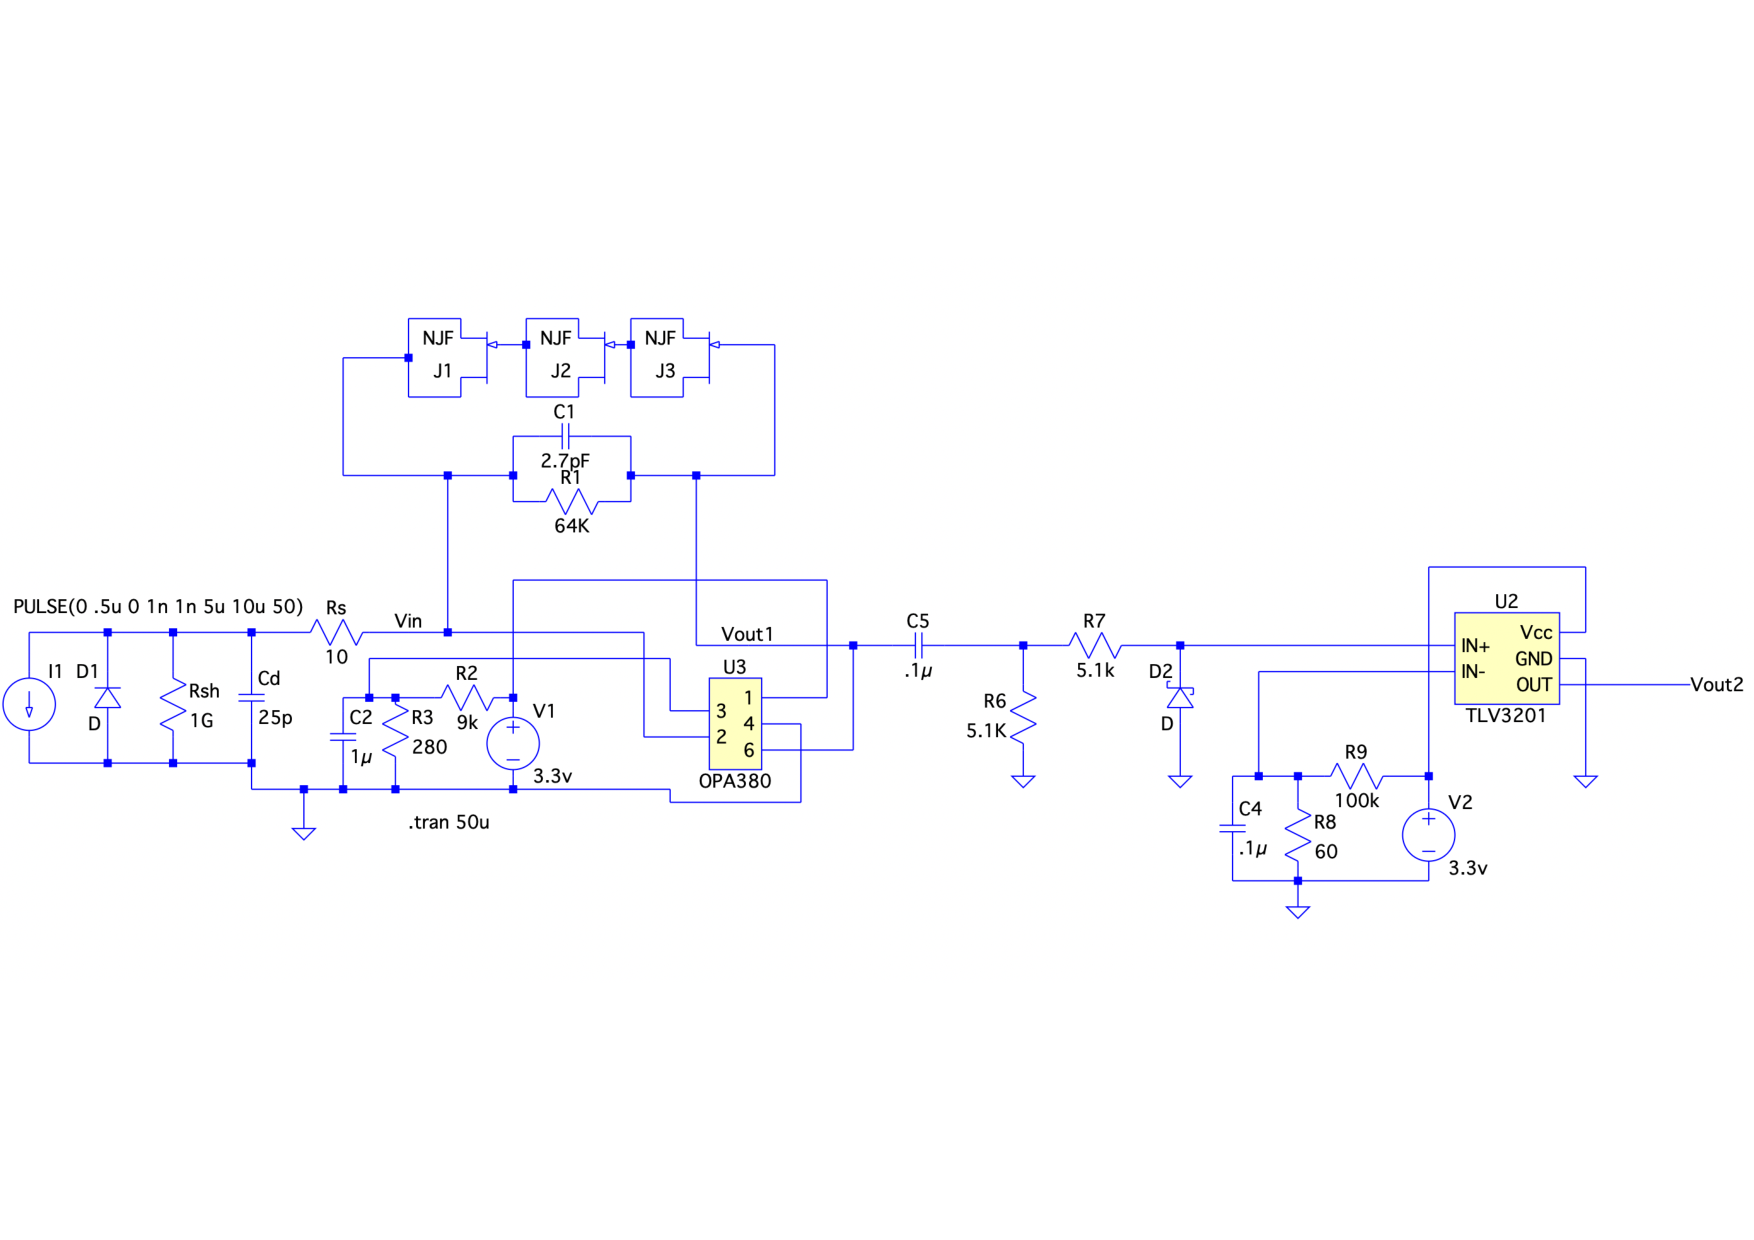
\includegraphics[width=0.75\linewidth]{fig/space_com_2.pdf}
    \caption{LTSpice model of Communication branch for Space Splitting.}
    \label{fig:4.11}
\end{figure}


\begin{figure}
    \centering
    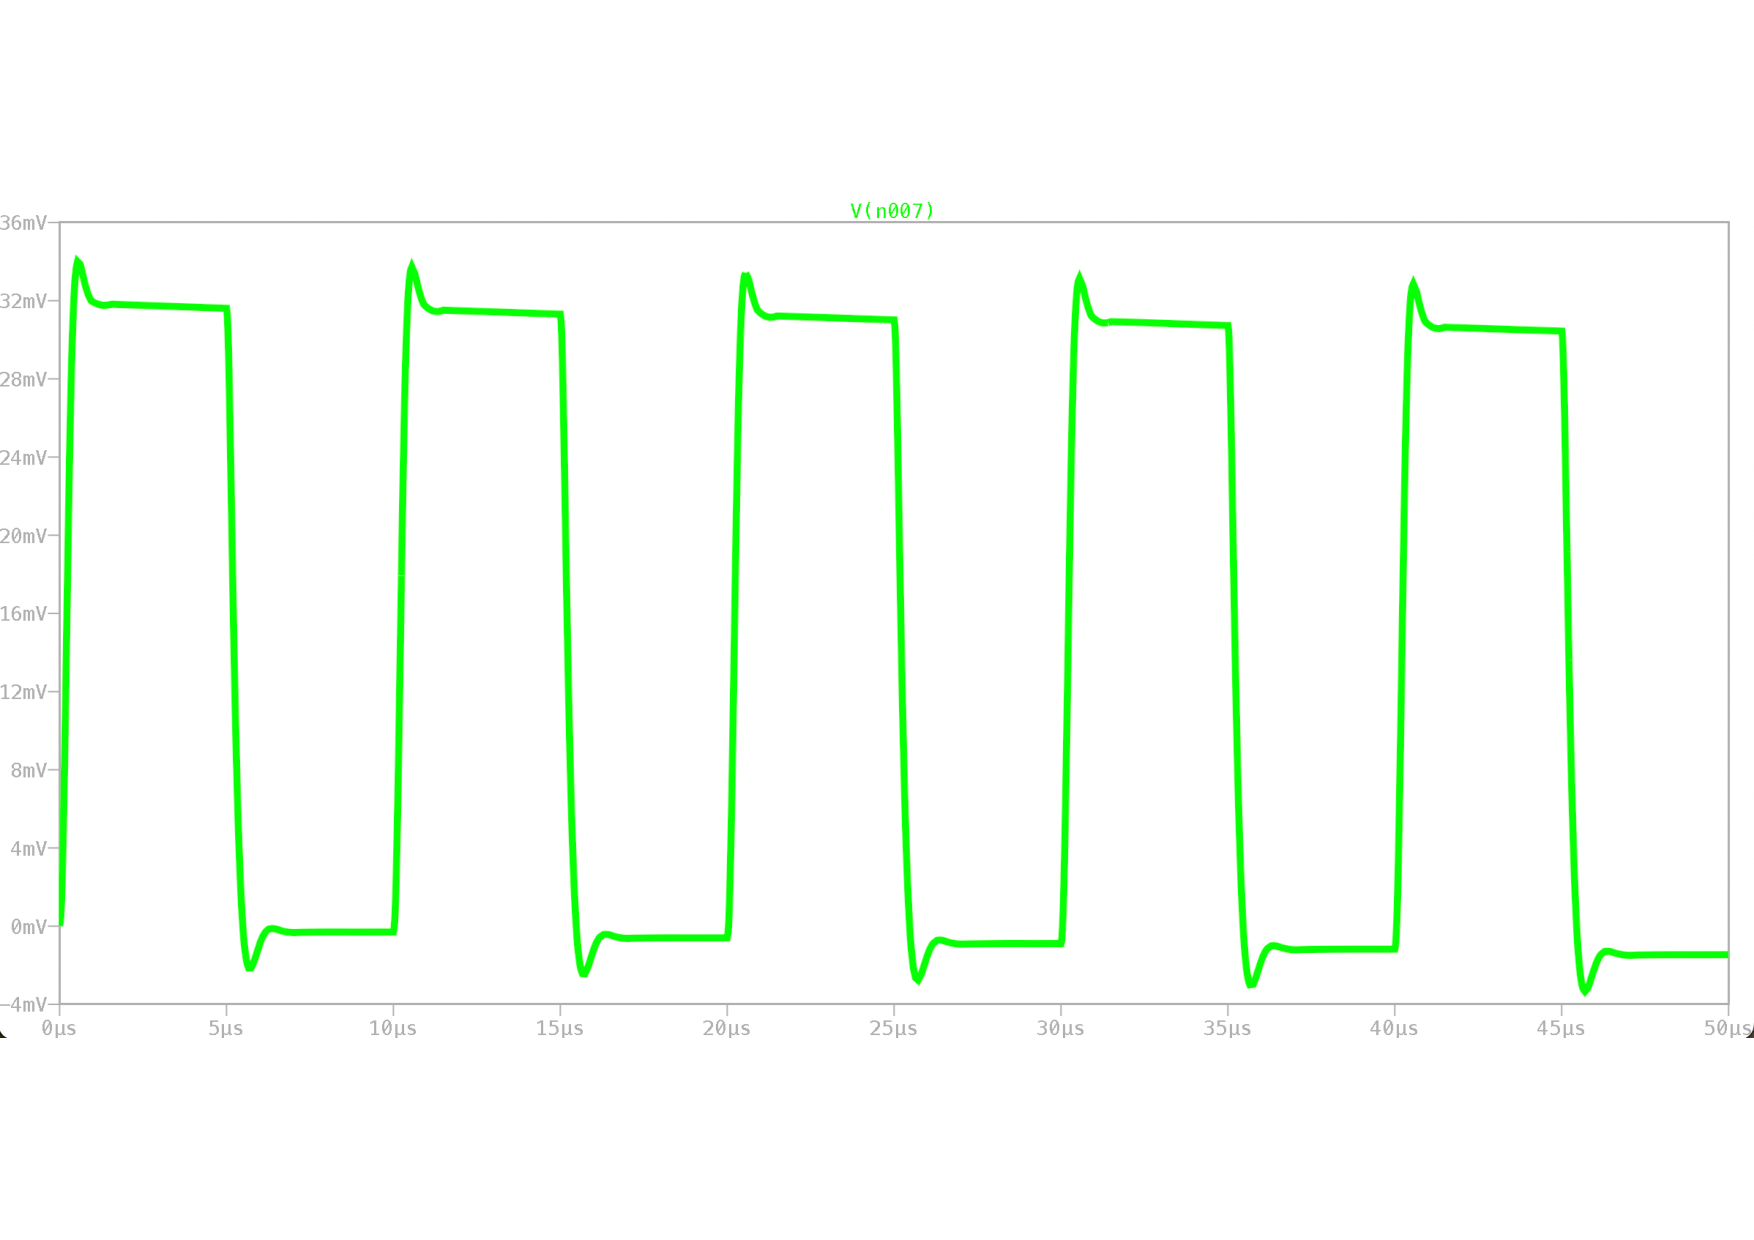
\includegraphics[width=0.75\linewidth]{fig/TIA output.pdf}
    \caption{Simulation Output of TIA.}
    \label{fig:4.12}
\end{figure}

As the pulse output ranges from 0 to 32 mV, shown in Figure \ref{fig:4.12}, the voltage reference is taken as 2 mV, against which the output from \ac{TIA} will be compared. From equation \ref{eq:3.21} and according to Figure \ref{fig:4.11}.

\begin{equation}
\ 2mV =  3.3 V \frac{ R_8 }{R_8 + R_9} \
\label{eq:4.19}
\end{equation}

Here, \(R_{9}\) taken as 100k\(\Omega\) as a standard as explained by \cite{sboa219}. Then the value of \(R_{8}\) becomes 60\(\Omega\). After putting this value into the LTSpice model and simulation, the output of the whole communication branch is shown in Figure \ref{fig:4.12}

\begin{figure}
    \centering
    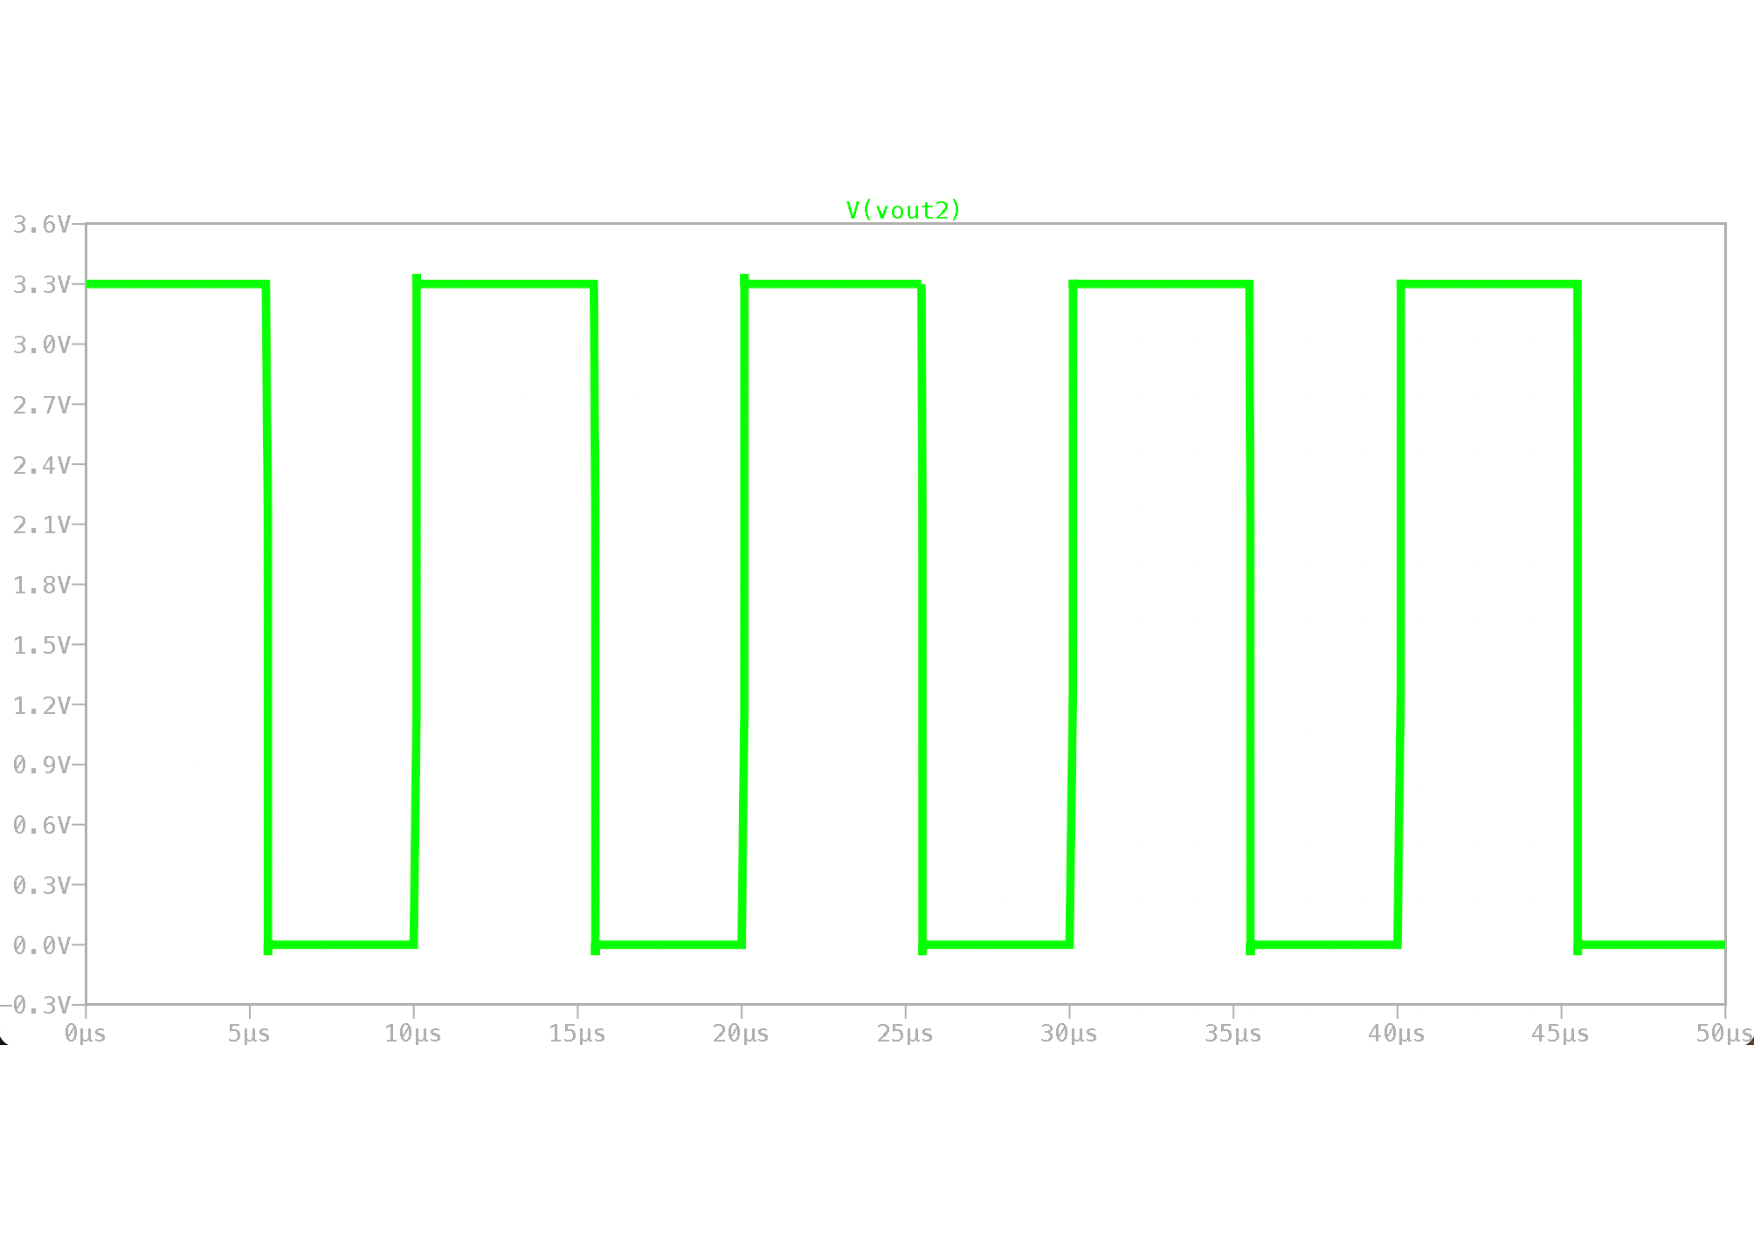
\includegraphics[width=0.75\linewidth]{fig/Comparator output.pdf}
    \caption{Simulation output of the communication branch for Space Splitting Technique.}
    \label{fig:4.13}
\end{figure}


After the validation from the simulation, the circuit design is put to work to build a real prototype. The circuit performs similarly to the simulation but contains much noise, and this is because of the real-world instruments and noises from the environment that are ever present. Again, this circuit is built on a breadboard, incorporating some resistance and capacitance. Some parameters are changed to reduce noise and have the optimum output from the \ac{TIA}. For example, feedback resistance and capacitance are changed into 100K\(\Omega\) and 9pF, respectively. Bias divider resistor \(R_{2}\) is taken 10K\(\Omega\) instead of 9K\(\Omega\). Filter resitors \(R_{6}\) and \(R_{7}\) are now each 6.8K\(\Omega\).

Another important fact is that the pulse output from the \ac{TIA} also goes below the zero line. With this current setup, a normal pulse response at a distance between the Transmitter and Receiver of 10cm, the output from \ac{TIA}(after filtering) goes from -19 mV to 21 mV. 

Although the pulse range is changed, the reference voltage for the comparator circuit is not changed, as it is still capable of comparing and turning the analog output from \ac{TIA} to digital output. That means the biasing voltage divider resistor circuit remains the same.

Then this digital output is fed to the selected STM32 Nucleo Board. The algorithm for coding the STM32 is shown in Figure \ref{fig:4.14}. STOP mode is chosen because it has a very low current consumption of 114 \(\mu\)A at 3.6V \cite{pwr}. Once the code is run, the STM32 MCU will run and initialize the peripherals. Then it will enter the STOP mode directly. It wakes up instantly once it receives data as an Interrupt from the comparator output. It gets the data as a byte and saves it onto a Buffer. Once Buffer is full, it sends the data to the PC via USART2 DMA. There is an inactivity checker running parallel to this primary function. Once no data is received within 30 seconds, the STM32 will return to STOP mode. 

\begin{figure}
    \centering
    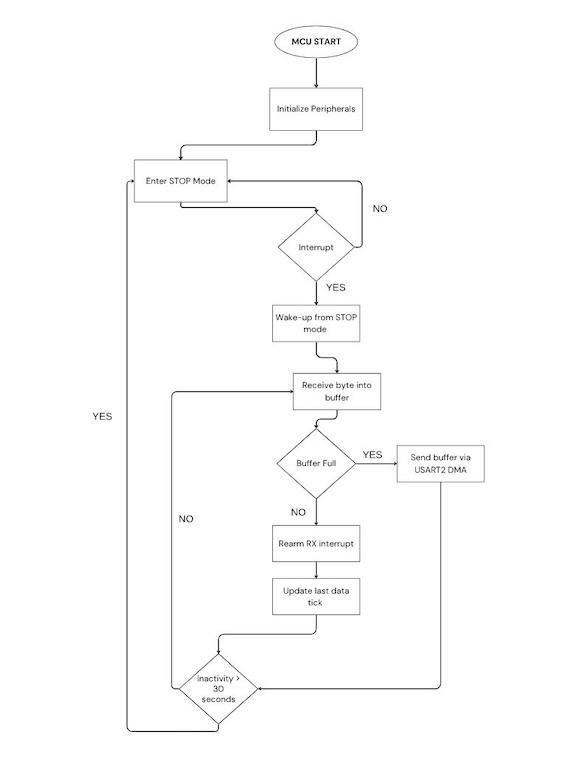
\includegraphics[width=0.75\linewidth]{fig/Algorithm .jpg}
    \caption{STM32 Programming Algorithm}
    \label{fig:4.14}
\end{figure}

\subsubsection{Energy Harvesting Brunch}

To start \ac{EH} with Solar Click \ac{EVM}, the minimum voltage and power required are 100 mV and 0.005 mW \cite{solar}, which means that the \ac{EH} source needs to produce 50 \(\mu\)A at least for regular operation. Again, cold start voltage is 600 mV and power is 15 \(\mu\)A, and even if for cold start, 25 \(\mu\)A is necessary\cite{slusbh2}

The \ac{EVM} supplies 2.6V and 100mA to the connected load at the output terminal \cite{solar}. This is low for this thesis's requirement, which is 3.3V. To achieve this, a resistor of the \ac{EVM} for output regulation needed to be changed.
The output regulation voltage equation given by \cite{slusbh2}:

\begin{equation}
\ V_{out} =  V_{Bias} \frac{ R_{out2} + R_{out1} }{R_{out2}} \
\label{eq:4.21}
\end{equation}

Here, \(V_{bias}\) given 1.21 V and \(V_{out}\) is 3.3 V then,
\begin{equation}
\ R_{out1} = 0.6 R_{out2} \
\label{eq:4.22}
\end{equation}

Since \(R_{out2}\) is 1M\(\Omega\) for the \ac{EVM} then by keeping it same \(R_{out1}\) becomes 600K\(\Omega\).

The overvoltage protection level was also raised to 5.1 V by changing the resistor \(R_{ov1}\) to 620K\(\Omega\). The calculation is taken from the datasheet of the BQ25570 datasheet\cite{solar}.

The final circuit design with both Energy harvesting and Communication Branch is shown in Figure \ref{fig:4.15}:

\begin{figure}
    \centering
    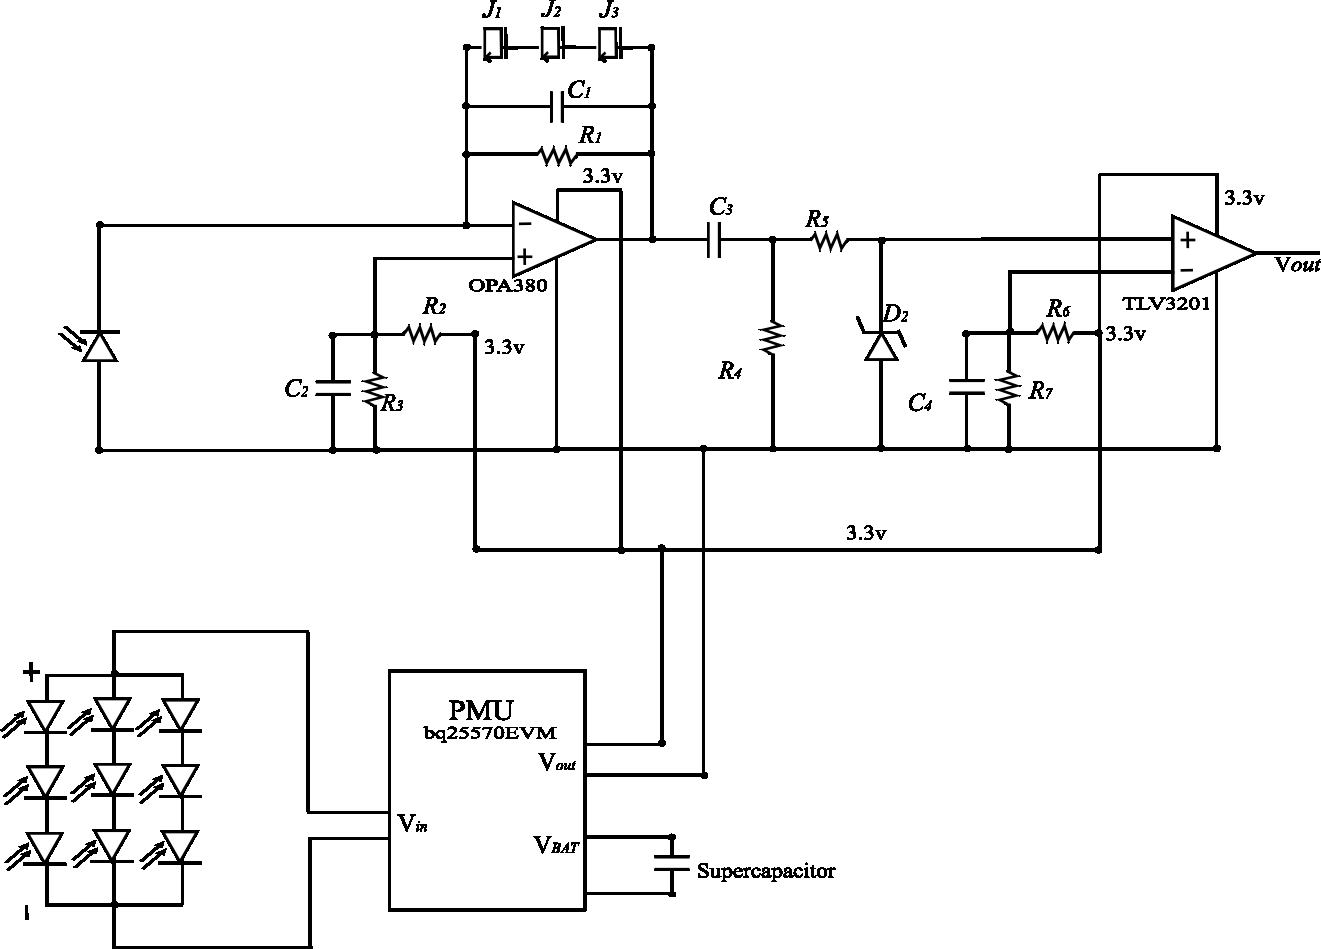
\includegraphics[width=0.75\linewidth]{fig/totalcircuit_3.jpg}
    \caption{Space Splitting Li-Fi receiver}
    \label{fig:4.15}
\end{figure}

\subsection{Power Splitting}

Light from the LED is fed to \ac{PD}s in series. Here, 12 BPW34 is soldered together to form an array shown in Figure \ref{fig:3.2}. Since they are in a series configuration, their output voltage is multiplied by twelve, but the current remains the same. The light illumination on the \ac{PD} is done in a confined box, which reduces ambient light. Since only artificial light(LED) is used, the I-V curve plotting will not be possible using the datasheet values. By varying the load, different current and voltage points are measured using a precision Multimeter. Then, the I-V curve is plotted, as shown in Figure \ref{fig:4.6}.

\begin{figure}
    \centering
    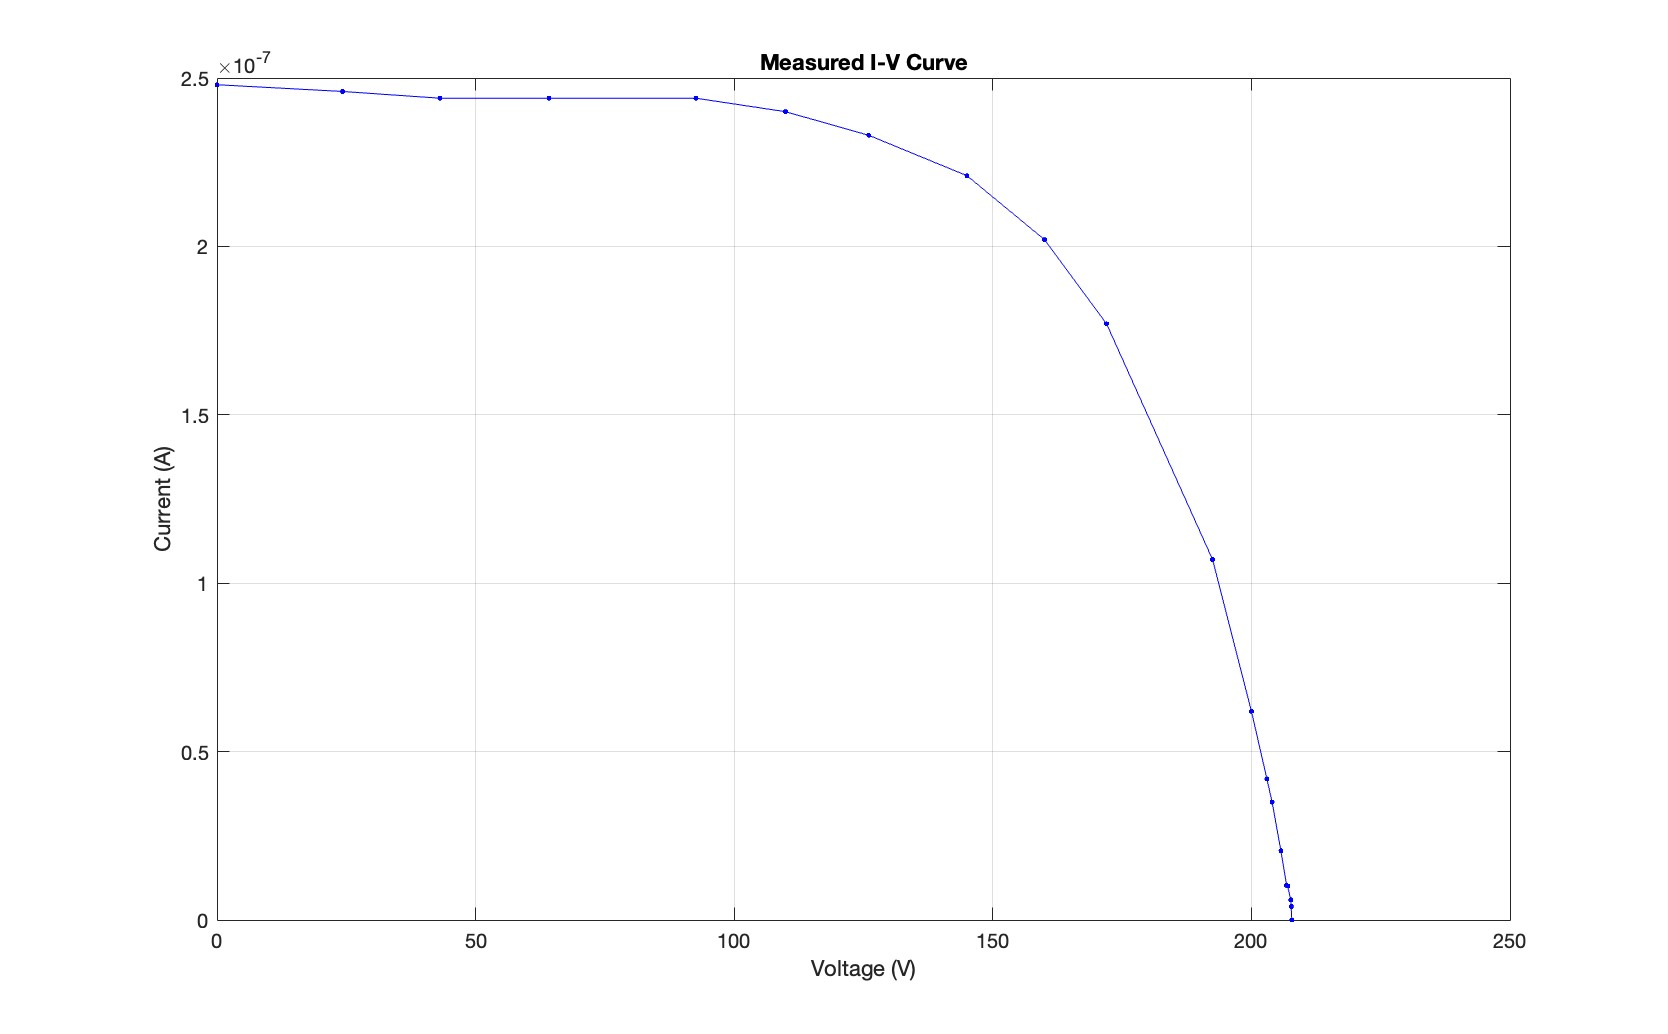
\includegraphics[width=0.75\linewidth]{fig/IV_Curve.jpg}
    \caption{I-V curve of the \ac{PD} in Photovoltaic Mode.}
    \label{fig:4.6}
\end{figure}

From the derivative of current to voltage at short circuit condition and using the equation \ref{eq:4.5}, the value of \(R_{sh}\) is found to be 12.15M \(\Omega\) and then using \ref{eq:3.8} it is found to be 145.8M \(\Omega\). By using a derivative of voltage to current at short circuit condition, and using the equation \ref{eq:4.8}, \(R_{s}\) is found to be negligible (\(\leq\).5\(\Omega\)). Since 12 \ac{PD}s are soldered in series, their total value is 12\(\Omega\).
According to the datasheet of the BPW34 diode, the capacitance is typically 70pF at zero biasing voltage, then the equivalent capacitance according to \ref{eq:3.9} becomes 5.83pF, but is taken as approx 7pF. The value of L is approximately taken as 130nF. Using \ref{eq:3.9}, small signal resistance is calculated as 700 \(\Omega\). 

However, since the required inductance was not available, the circuit was reconfigured only with resistors and capacitors. In principle, an RC filter of a Lower cutoff frequency is designed for the Communication branch to eliminate values close to DC, and a High cutoff frequency filter for the Energy Harvest branch to eliminate AC values.

\subsubsection{Simulation}

The values of the five parameters are then applied to the LTSpice circuit to find other circuit parameters. The redesigned circuit is shown in Figure \ref{fig:4.7}. A step parameter command with AC analysis is performed to find the optimum values. A voltage amplifier with a comparator circuit is also designed in LTSpice and simulated, shown in Figure \ref{fig:4.8}.

\begin{figure}
    \centering
    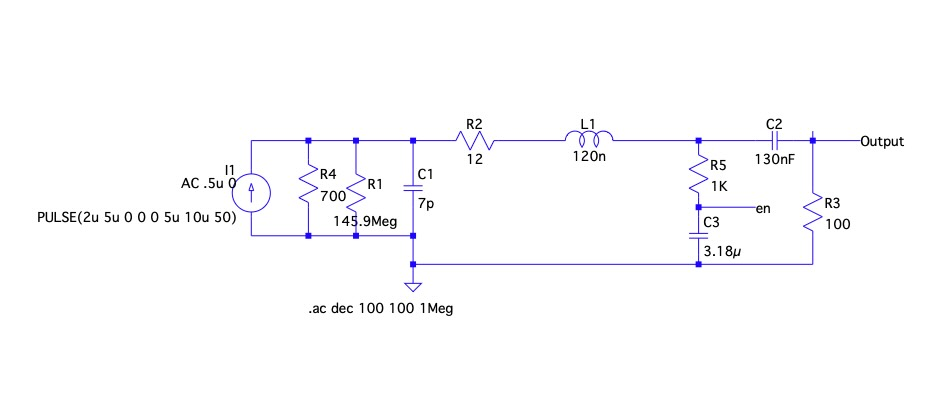
\includegraphics[width=1\linewidth]{fig/LTSpice filter.jpg}
    \caption{Redesigned AC-DC separation circuit in LTSpice.}
    \label{fig:4.7}
\end{figure}


\begin{figure}
    \centering
    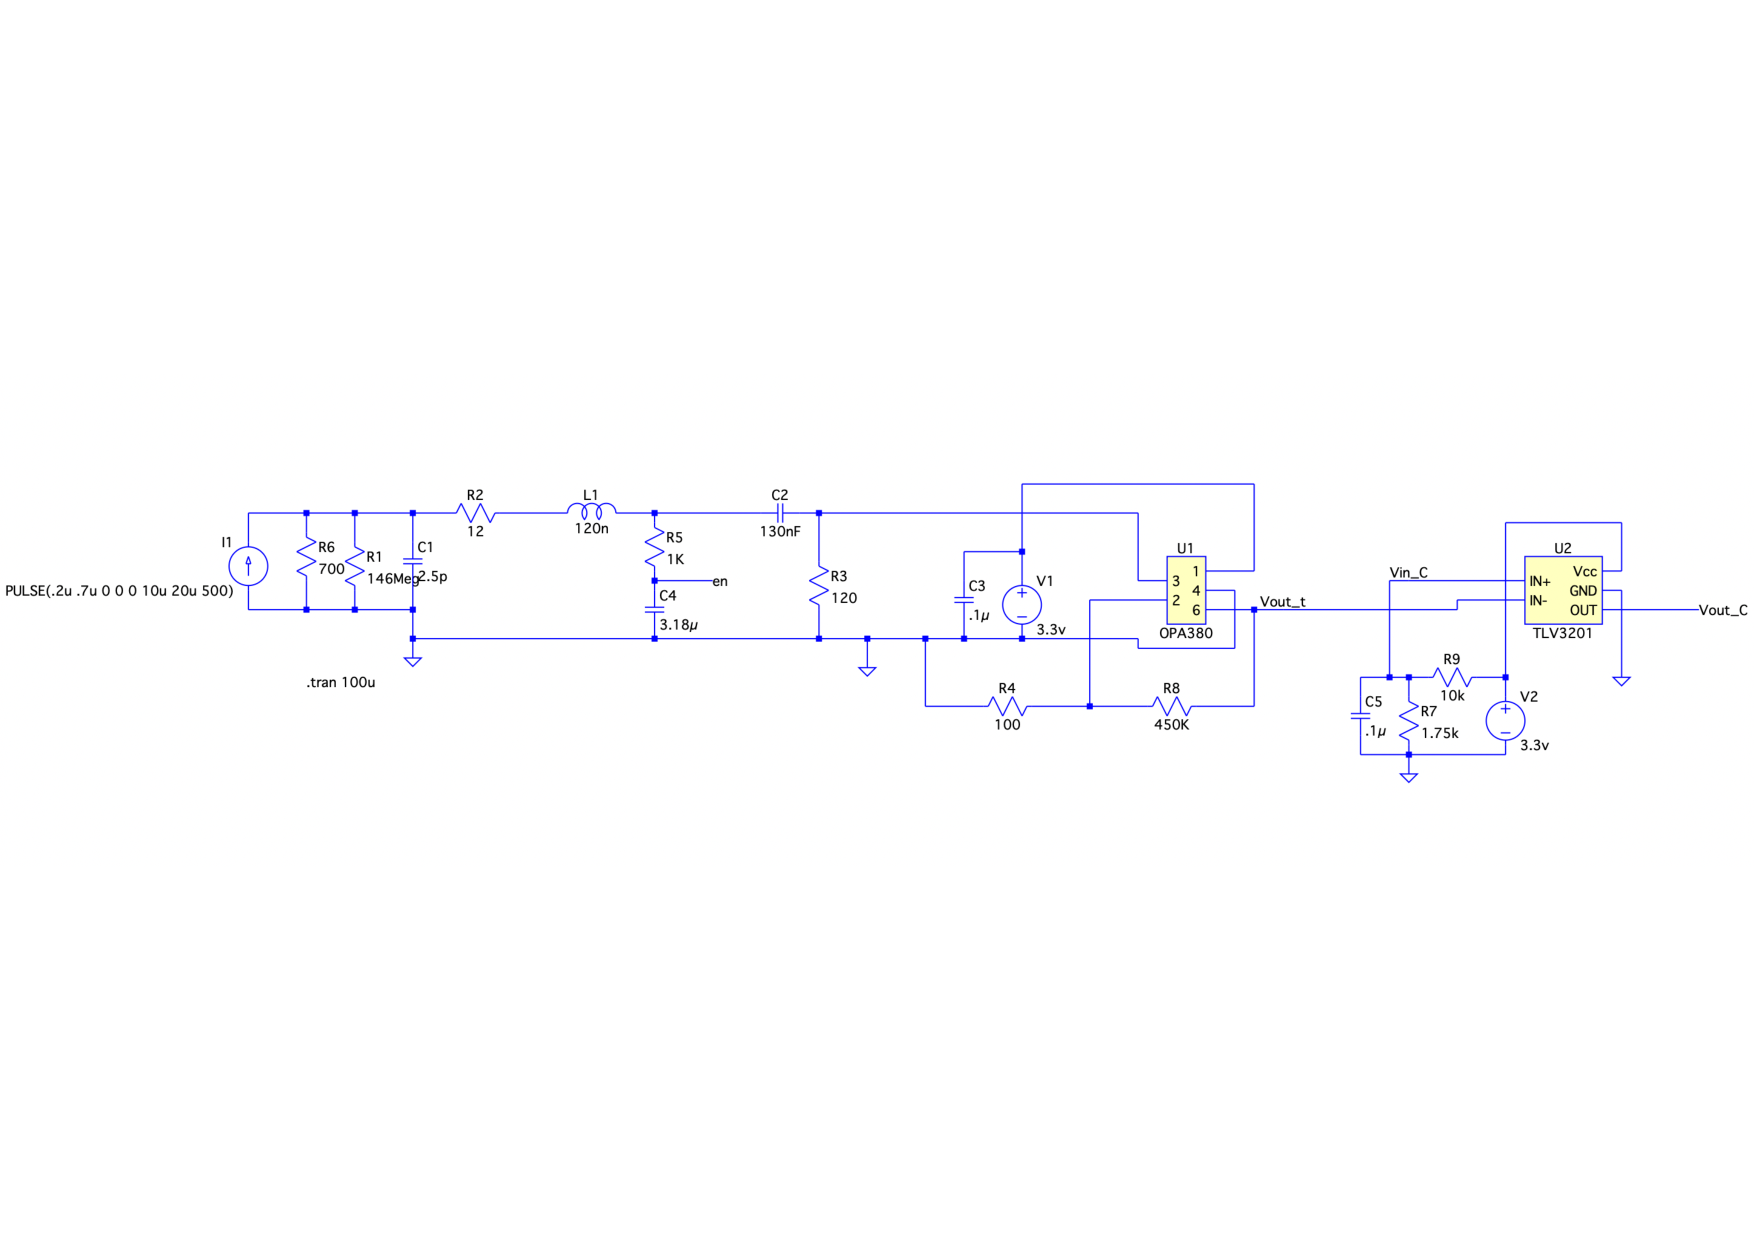
\includegraphics[width=1\linewidth]{fig/powersplit com.pdf}
    \caption{LTSpice Communication Branch design for \ac{PS}.}
    \label{fig:4.8}
\end{figure}

\begin{figure}
    \centering
    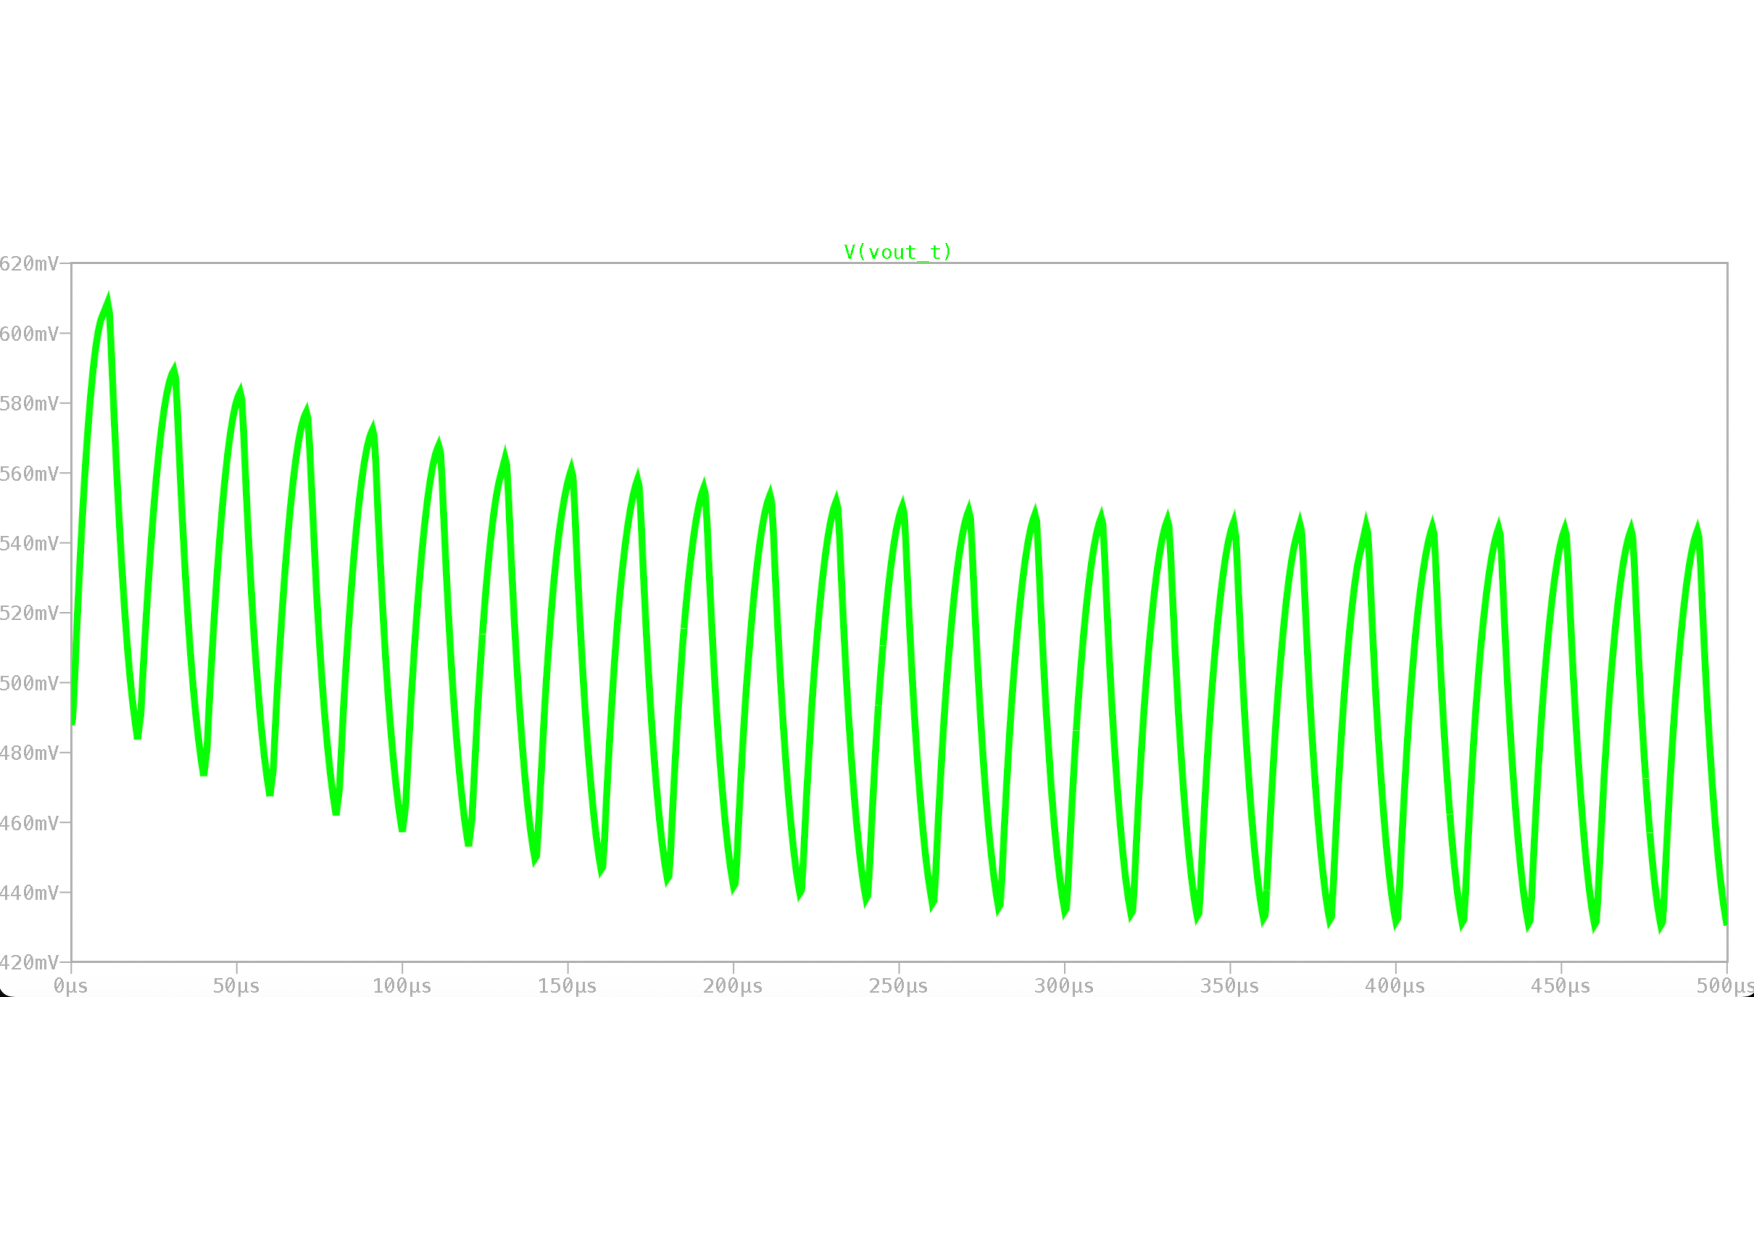
\includegraphics[width=0.75\linewidth]{fig/power_amplifier res.pdf}
    \caption{Communication Branch Amplifier Response}
    \label{fig:4.9}
\end{figure}

\begin{figure}
    \centering
    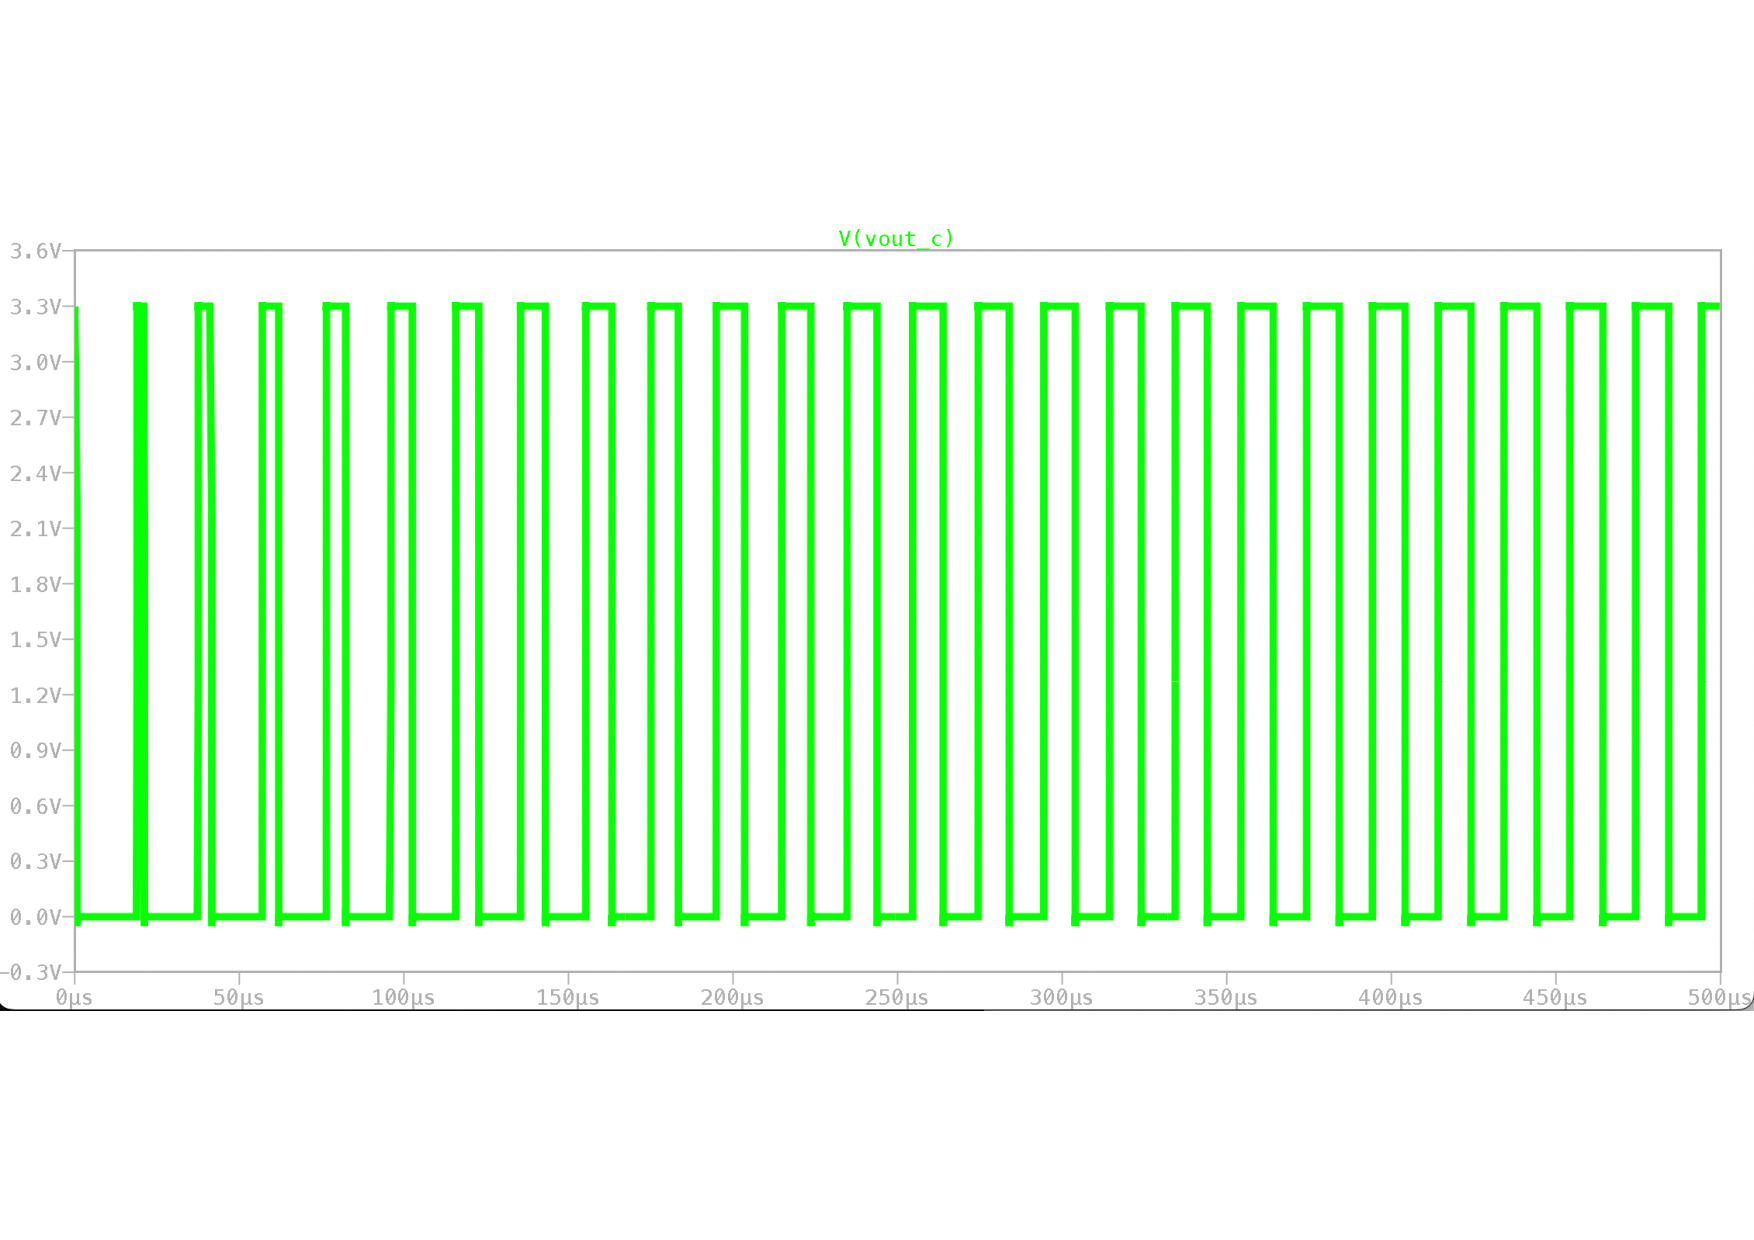
\includegraphics[width=0.75\linewidth]{fig/power_com_res.pdf}
    \caption{Communication Branch comparator Response}
    \label{fig:4.10}
\end{figure}

Figure \ref{fig:4.9} shows the simulated amplifier pulse response. At first, the response took 180 \(\mu\)S to settle down, and it was constantly between 570 mV and 435 mV. Simulated comparator response is also shown in Figure \ref{fig:4.10}. At first, the pulse width was smaller than the rest, which reduced after 180 \(\mu\)S.